% 若编译失败,且生成 .synctex(busy) 辅助文件,可能有两个原因:
% 1. 需要插入的图片不存在:Ctrl + F 搜索 'figure' 将这些代码注释/删除掉即可
% 2. 路径/文件名含中文或空格:更改路径/文件名即可

% --------------------- 文章宏包及相关设置 --------------------- %
% >> ------------------ 文章宏包及相关设置 ------------------ << %
% 设定文章类型与编码格式
\documentclass[zihao=-4, UTF8]{article}		% 设置全文字号大小, -4 为小四, 5 为五号

% 本文特殊宏包

% 自定义宏定义
    \def\N{\mathbb{N}}
    \def\F{\mathbb{F}}
    \def\Z{\mathbb{Z}}
    \def\Q{\mathbb{Q}}
    \def\R{\mathbb{R}}
    \def\C{\mathbb{C}}
    \def\T{\mathbb{T}}
    \def\S{\mathbb{S}}
    \def\A{\mathbb{A}}
    \def\I{\mathscr{I}}
    \def\d{\mathrm{d}}
    \def\p{\partial}


% 导入基本宏包
    \usepackage[UTF8]{ctex}     % 设置文档为中文语言
    \usepackage[colorlinks, linkcolor=blue, anchorcolor=blue, citecolor=blue, urlcolor=blue]{hyperref}  % 宏包:自动生成超链接 (此宏包与标题中的数学环境冲突)
    % \usepackage{docmute}    % 宏包:子文件导入时自动去除导言区,用于主/子文件的写作方式,\include{./51单片机笔记}即可。注:启用此宏包会导致.tex文件capacity受限。
    \usepackage{amsmath,amssymb,amsfonts}  % 宏包:更多数学公式和数学符号
    \usepackage{mathrsfs}   % 宏包:提供更多数学符号
    \usepackage{pifont}     % 宏包:提供了特殊符号和字体
    \usepackage{extarrows}  % 宏包:更多箭头符号
    \usepackage{multicol}   % 宏包:支持多栏 



% 文章页面margin设置
    \usepackage[a4paper]{geometry}
        \geometry{top=2.6cm}  % 1 inch= 2.46 cm, 0.75 inch = 1.85 cm
        \geometry{bottom=2.6cm}
        \geometry{left=2.55cm}
        \geometry{right=2.55cm}   % 设置上下左右页边距
        \geometry{marginparwidth=1.75cm}    % 设置边注距离(注释、标记等)

% 配置数学环境
    \usepackage{amsthm} % 宏包:数学环境配置
    % theorem-line 环境自定义
        \newtheoremstyle{MyLineTheoremStyle}% <name>
            {11pt}% <space above>
            {11pt}% <space below>
            {}% <body font> 使用默认正文字体
            {}% <indent amount>
            {\bfseries}% <theorem head font> 设置标题项为加粗
            {:}% <punctuation after theorem head>
            {.5em}% <space after theorem head>
            {\textbf{#1}\thmnumber{#2}\ \ (\,\textbf{#3}\,)}% 设置标题内容顺序
        \theoremstyle{MyLineTheoremStyle} % 应用自定义的定理样式
        \newtheorem{LineTheorem}{Theorem.\,}
    % theorem-block 环境自定义
        \newtheoremstyle{MyBlockTheoremStyle}% <name>
            {11pt}% <space above>
            {11pt}% <space below>
            {}% <body font> 使用默认正文字体
            {}% <indent amount>
            {\bfseries}% <theorem head font> 设置标题项为加粗
            {:\\ \indent}% <punctuation after theorem head>
            {.5em}% <space after theorem head>
            {\textbf{#1}\thmnumber{#2}\ \ (\,\textbf{#3}\,)}% 设置标题内容顺序
        \theoremstyle{MyBlockTheoremStyle} % 应用自定义的定理样式
        \newtheorem{BlockTheorem}[LineTheorem]{Theorem.\,} % 使用 LineTheorem 的计数器
    % definition 环境自定义
        \newtheoremstyle{MySubsubsectionStyle}% <name>
            {11pt}% <space above>
            {11pt}% <space below>
            {}% <body font> 使用默认正文字体
            {}% <indent amount>
            {\bfseries}% <theorem head font> 设置标题项为加粗
            {:\\ \indent}% <punctuation after theorem head>
            {0pt}% <space after theorem head>
            {\textbf{#3}}% 设置标题内容顺序
        \theoremstyle{MySubsubsectionStyle} % 应用自定义的定理样式
        \newtheorem{definition}{}

%宏包:有色文本框(proof环境)及其设置
    \usepackage[dvipsnames,svgnames]{xcolor}    %设置插入的文本框颜色
    \usepackage[strict]{changepage}     % 提供一个 adjustwidth 环境
    \usepackage{framed}     % 实现方框效果
        \definecolor{graybox_color}{rgb}{0.95,0.95,0.96} % 文本框颜色。修改此行中的 rgb 数值即可改变方框纹颜色,具体颜色的rgb数值可以在网站https://colordrop.io/ 中获得。(截止目前的尝试还没有成功过,感觉单位不一样)(找到喜欢的颜色,点击下方的小眼睛,找到rgb值,复制修改即可)
        \newenvironment{graybox}{%
        \def\FrameCommand{%
        \hspace{1pt}%
        {\color{gray}\small \vrule width 2pt}%
        {\color{graybox_color}\vrule width 4pt}%
        \colorbox{graybox_color}%
        }%
        \MakeFramed{\advance\hsize-\width\FrameRestore}%
        \noindent\hspace{-4.55pt}% disable indenting first paragraph
        \begin{adjustwidth}{}{7pt}%
        \vspace{2pt}\vspace{2pt}%
        }
        {%
        \vspace{2pt}\end{adjustwidth}\endMakeFramed%
        }

% 外源代码插入设置
    % matlab 代码插入设置
    \usepackage{matlab-prettifier}
        \lstset{
            style=Matlab-editor,  % 继承matlab代码颜色等
        }
    \usepackage[most]{tcolorbox} % 引入tcolorbox包 
    \usepackage{listings} % 引入listings包
        \tcbuselibrary{listings, skins, breakable}
        \lstset{
            language=Matlab,
            basicstyle=\small,
            breakatwhitespace=false,
            breaklines=true,
            captionpos=b,
            keepspaces=true,
            numbers=left,
            numbersep=15pt,
            showspaces=false,
            showstringspaces=false,
            showtabs=false,
            tabsize=2,
            frame=single,
            frameround=tttt,
        }
        \lstdefinestyle{matlabstyle}{
            language=Matlab,
            basicstyle=\small,
            breakatwhitespace=false,
            breaklines=true,
            captionpos=b,
            keepspaces=true,
            numbers=left,
            numbersep=15pt,
            showspaces=false,
            showstringspaces=false,
            showtabs=false,
            tabsize=2,
        }
        \newtcblisting{matlablisting}{
            arc=0pt,
            top=0pt,
            bottom=0pt,
            left=1mm,
            listing only,
            listing style=matlabstyle,
            breakable,
            colback=white   % 选一个合适的颜色
        }

% table 支持
    \usepackage{booktabs}   % 宏包:三线表
    \usepackage{tabularray} % 宏包:表格排版
    \usepackage{longtable}  % 宏包:长表格

% figure 设置
    \usepackage{subcaption} % 用于子图和小图注  
    \usepackage{graphicx}  % 支持 jpg, png, eps, pdf 图片 
    \usepackage{svg}       % 支持 svg 图片
        \svgsetup{
            % 指向 inkscape.exe 的路径
            inkscapeexe = D:/aa_my_apps_main/Inkscape/bin/inkscape.exe, 
            % 一定程度上修复导入后图片文字溢出几何图形的问题
            inkscapelatex = false                 
        }

% 图表进阶设置
    \usepackage{caption}    % 图注、表注
        \captionsetup[figure]{name=图}  
        \captionsetup[table]{name=表}
        \captionsetup{labelfont=bf, font=small}
    \usepackage{float}     % 图表位置浮动设置 

% 圆圈序号自定义
    \newcommand*\circled[1]{\tikz[baseline=(char.base)]{\node[shape=circle,draw,inner sep=0.8pt, line width = 0.03em] (char) {\small \bfseries #1};}}   % TikZ solution

% 列表设置
    \usepackage{enumitem}   % 宏包:列表环境设置
        \setlist[enumerate]{
            label=(\arabic*),
            ref=\arabic*,
            itemsep=0pt, parsep=0pt, topsep=0pt, partopsep=0pt, leftmargin=3.5em} 
        \setlist[itemize]{itemsep=0pt, parsep=0pt, topsep=0pt, partopsep=0pt, leftmargin=3.5em}
        \newlist{circledenum}{enumerate}{1} % 创建一个新的枚举环境  
        \setlist[circledenum,1]{  
            label=\protect\circled{\arabic*}, % 使用 \arabic* 来获取当前枚举计数器的值,并用 \circled 包装它  
            ref=\arabic*, % 如果需要引用列表项,这将决定引用格式(这里仍然使用数字)
            itemsep=0pt, parsep=0pt, topsep=0pt, partopsep=0pt, leftmargin=3.5em
        }  

% 其它设置
    % 脚注设置
        \renewcommand\thefootnote{\ding{\numexpr171+\value{footnote}}}
    % 参考文献引用设置
        \bibliographystyle{unsrt}   % 设置参考文献引用格式为unsrt
        \newcommand{\upcite}[1]{\textsuperscript{\cite{#1}}}     % 自定义上角标式引用
    % 文档摘要设置
        \newcommand{\cnabstractname}{\large 摘要}
        \newenvironment{cnabstract}{%
        \par
        \noindent\mbox{}\hfill{\bfseries \cnabstractname}\hfill\mbox{}\par
        }{\par}

% 文章默认字体设置
\usepackage{fontspec}   % 宏包:字体设置
    \setmainfont{SimSun}    % 设置中文字体为宋体字体
    \setCJKmainfont[AutoFakeBold=3]{SimSun} % 设置加粗字体为 SimSun 族,AutoFakeBold 可以调整字体粗细
    \setmainfont{Times New Roman} % 设置英文字体为Times New Roman

% 各级标题自定义设置
\usepackage{titlesec} % 宏包:各级标题设置
\usepackage{titling}  % 宏包:标题设置
\setlength{\droptitle}{-2.6cm}  % 调整标题位置
\pretitle{\begin{center}\LARGE}
\posttitle{\end{center}}
% section标题自定义设置 
\titleformat{\section}{\Large\centering\bfseries}{\thesection.}{1em}{}
\titleformat{\subsection}{\normalsize\large\bfseries}{\thesubsection}{1em}{}
\titleformat{\subsubsection}{\normalsize\bfseries}{\thesubsubsection}{1em}{}
% subsubsection标题自定义设置
%\titleformat{\subsubsection}[hang]{\normalfont\bfseries}{}{8pt}{}

% --------------------- 文章宏包及相关设置 --------------------- %
% >> ------------------ 文章宏包及相关设置 ------------------ << %

% ------------------------ 文章信息区 ------------------------ %
% ------------------------ 文章信息区 ------------------------ %
% 页眉页脚设置
    %\usepackage{fancyhdr}   %宏包:页眉页脚设置
    %    \pagestyle{fancy}
    %    \fancyhf{}
    %    \cfoot{\thepage}
    %    \renewcommand\headrulewidth{1pt}
    %    \renewcommand\footrulewidth{0pt}
    %    \lhead{2024.8-2025.1} 
    %    \chead{here is the header,这里是页眉}    
    %    \rhead{dingyi233@mails.ucas.ac.cn}
%文档信息设置
    \title{\textbf{“板凳长龙”机理建模与设计优化}}
    \author{ }  % 必须为空
    \date{ }  % 必须为空
% ------------------------ 文章信息区 ------------------------ %
% ------------------------ 文章信息区 ------------------------ %

% 开始编辑文章

\begin{document} 

\maketitle
%\thispagestyle{fancy}
\vspace{-80pt}

\begin{cnabstract}
    {\normalsize 
        “板凳龙”,是起源于我国河洛地区的一种传统民俗活动,是我国南方许多省市的元宵庆祝活动之一,有丰富的文化内涵。本文主要分析了舞龙过程,研究舞龙路径、龙头速度等参数对舞龙过程的影响,建立了\textbf{基于刚体限制的舞龙队模型},并利用\textbf{变步长搜索}、\textbf{二分法}、\textbf{模拟退火}等方法进行求解。\par
        \textbf{针对问题一:}我们建立了\textbf{舞龙队位置速度模型}。首先,引入阿基米德螺线,以螺线起点为原点建立极坐标系,得到螺线方程为$r(\theta)=b\theta$。以盘入瞬间为时间原点,建立时间 $t$ 与龙头前把手极角 $\theta_0$ 之间的函数关系,以此求出龙头前把手的位置,并利用刚体限制,\textbf{将变步长搜索与二分法结合},计算出所有把手的位置。然后,计算各把手所在位置的切线方向和各板凳方向,由刚体限制推导出速度计算公式,最终得到所有把手的位置和速度结果。
        %例如,$t$ = 300 s 时,\textbf{龙尾后把手位置和速度分别为 (1.785033\ m, 9.301164\ m) 和 0.996478 $\mathbf{m\cdot s^{-1}}$},其余
        结果详见表 \ref*{问题1位置结果} 、表 \ref*{问题1速度结果} 和文件 \textbf{result1.xlsx}。\par
        \textbf{针对问题二:}证明了只需考虑第一、二块板凳是否与其他板凳发生碰撞,我们建立了\textbf{舞龙队碰撞检测模型}和两种\textbf{最小螺距计算模型},结合变步长搜索和二分法,求解舞龙队盘入的终止时刻。在问题一的基础上,先确定所有板凳的位置信息,然后基于舞龙队碰撞检测模型,用变步长搜索对时间进行两轮迭代,将第一次碰撞时间锁定在较精确的小区间内,以确保没有漏过某次碰撞,且此区间不会出现其它碰撞情况。最后,借助二分法,求出终止时刻的精确值。得到碰撞时间为 \textbf{412.473838 s},其它计算结果详见文件 \textbf{result2.xlsx}。\par
        \textbf{针对问题三:}在问题二的基础上,建立了\textbf{螺距参数可调的舞龙队碰撞检测模型}。问题三的本质与问题二相同,只是螺距参数可调,以便于对不同螺距下的舞龙队进行碰撞检测。只需要改变螺距的值,求解出碰撞时刻的极径长度,与调头空间半径作对比,即可得到最终结果。考虑到时间坐标离散带来的误差影响,在实际解题过程中,我们采用了两种不同的做法:\textbf{二分法}、\textbf{模拟退火法}进行求解,两种方法得到的最小螺距分别为 $\mathbf{0.450337\ m}$ 和 $\mathbf{0.450297\ m}$。\par
        \textbf{针对问题四:}建立\textbf{调头位置可变的全路径舞龙队位置速度模型},并求解出满足刚体限制的\textbf{最小调头半径为 4.254674 m} 。为了保持精度的同时简便计算,规定实际调头路径起始点和终止点呈中心对称,由此可证\textbf{调头路线形状唯一确定},随后根据调头路线形状,确定了全路径在直角坐标系下的参数方程,并在编程过程中对不同把手所处不同曲线进行区分,最终得出所需时间段内各把手的位置速度信息,计算结果详见文件 \textbf{result4.xlsx}。\par
        \textbf{针对问题五:}在问题四中模型的基础上,考虑速度大小限制条件,对龙头行进速度进行递减迭代,最终求得满足速度限制的\textbf{最大龙头行进速度为} $\mathbf{0.409122\  m\cdot s^{-1}}$。

        \par
    }\par
    \vspace{12pt}
    {\normalsize \textbf{关键词: 阿基米德螺线,刚体限制,变步长搜索法,二分法,模拟退火}}
\end{cnabstract}
\setlength{\parindent}{2em}

\newpage
\section{问题重述}

板凳龙,是起源于我国河洛地区的传统民俗活动,是百姓迎神祈福的重要活动之一。板凳龙表演过程中有“盘龙”的舞蹈动作,我们对盘龙路线与相关参数建立了\textbf{基于刚体限制}的高精度数学模型,并以此通过计算解决以下问题。\par
\begin{figure}[H]\centering
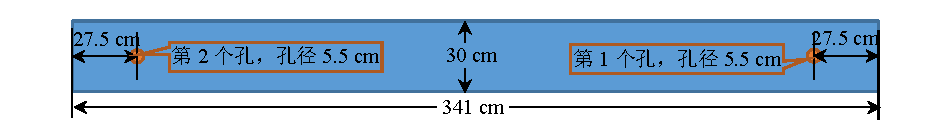
\includegraphics[width=\textwidth]{assets/dragonhead.pdf}
\caption{\bfseries 龙头俯视图}\label{龙头俯视图}
\end{figure}
\begin{figure}[H]\centering
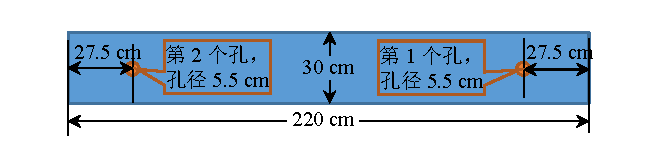
\includegraphics[width=0.7\textwidth]{assets/dragonbody.pdf}
\caption{\bfseries 龙身俯视图}\label{龙身俯视图}
\end{figure}
\textbf{问题一:}“板凳龙”的行进路线是一条螺距为 $55\ \mathrm{cm}$ 的 阿基米德螺线,龙头为特殊的板凳,其它所有板凳有完全一致的结构,且相邻把手是等间距的(龙头前后把手除外),龙头从特定起点开始,沿阿基米德螺线匀速前进。以开始盘入为时间起点,求出 0 s $\sim$ 300 s 时间段内,每秒整个舞龙队的的位置和速度。将最终结果保留 6 位小数,写入到文件 result1.xlsx 中,在论文中以表格形式给出部分结果。\par
\textbf{问题二:}舞龙队沿问题 1 设定的螺线路径盘入,以板凳之间不发生碰撞为限制,计算盘入的终止时刻,即发生第一次碰撞的前一瞬间。记录此时舞龙队的具体位置与速度,将结果写入文件 result2.xlsx。\par
\textbf{问题三:}舞龙队从盘入到盘出需要一定的调头空间,调头空间是一个直径 9 m、圆心位于螺线中心的圆,求解最小螺距,使得龙头前把手能够进入调头空间。\par
\textbf{问题四:}舞龙队需要在调头空间内完成调头,调头路径由两段半径比为 2:1 且相连为 S 形的圆弧构成,且与盘入盘出螺线相切。确定调头路径,并调整圆弧,使得调头曲线变短。然后设定龙头前把手速度为 1 $\mathrm{m\cdot s^{-1}}$,给出调头前后时间段内,舞龙队的位置和速度。将结果保存到文件 result4.xlsx。\par
\textbf{问题五:}队伍沿问题 4 设定路径前行,龙头行进速度保持不变,队伍各把手速度均不超过 2 $\mathrm{m\cdot s^{-1}}$,求解龙头的最大行进速度。

\section{问题分析}
\subsection{问题一分析}
对于问题一,题目已经给出“板凳龙”的行进路线是一条\textbf{阿基米德螺线},考虑到阿基米德螺线的特性,我们考虑以曲线出发点为原点建立极坐标系,得到路径曲线方程为$r=b\theta$,其中 $b$ 由螺距确定。根据题目描述可知,除龙头上的两个把手外,其它所有相邻把手间都是等距的,所以只需要先求出第一、二块板凳的把手的位置,即沿用同样的思路,确定后续每个把手任意时刻的位置。由\textbf{刚体限制}推导出速度计算公式,并代入位置结果,就能求出所需的速度信息。

\subsection{问题二分析}
对于问题二,我们需要在问题一的基础上进行扩展。在问题一中,我们仅考虑了不同时刻下每个把手在阿基米德螺线上的位置和速度信息。在问题二中,我们需要根据每一对相邻把手的方向(板凳方向),\textbf{定位出其矩形位置}(板凳位置),这样就能模拟出板凳的全部信息,以便\textbf{建立碰撞检测模型}。又因为板凳龙中自第三个板凳开始,每一个板凳都一定会重复第二块板凳的运动,再结合盘入螺线的对称性,只需考虑的龙头和第二块板凳的外边缘棱角是否会同外圈板凳发生碰撞即可。因为题目要确定碰撞的时刻,我们考虑采用\textbf{变步长搜索法},对行进时间 $t$ 进行变步长迭代,并判断每步迭代后是否会发生碰撞。确定第一次碰撞时间后,回退多段时间防止漏测,再缩小步长进行二次迭代,以确定碰撞时间所在的小区间,最后利用\textbf{二分法},二分碰撞时间,并根据是否碰撞的条件缩小时间范围,以达成优化精度的目的。

\subsection{问题三分析}
问题三的本质和问题二是完全一致的。对于问题三,我们只需改变螺距这一参数,重复问题二的计算过程以得到碰撞时龙头距原点的距离,与调头空间半径作比较,若在进入调头区域前不发生碰撞则符合题意。

在确定螺距的具体实现过程中,考虑到时间离散所带来的检测误差,我们采用\textbf{二分法和模拟退火两种不同方法}进行解答。对于二分法,作出图像后可以发现,在调头空间半径附近,碰撞时的半径随螺距大小的变化是\textbf{严格单调}的,所以很容易想到利用二分法快速解题。但为了防止遗漏某些情况,我们还可以采用模拟退火法,在一定范围内对螺距进行迭代,以搜寻最小螺距,其优点是可以自动寻找全局最优解,降低了陷入局部最优解的概率。
\subsection{问题四分析}
问题四分为两个部分。对于第一部分,需要考虑到进入调头空间后,板凳龙仍可以\textbf{继续沿螺线行进一段距离再开始调头},也即在调头空间完成调头即可,并不是进入调头空间瞬间便开始调头。虽然实际调头路径的起始点和中止点可以不中心对称,但是这样会导致全路径曲线的参数方程求解困难。为了保持计算精度的同时,尽可能地简便计算,在后续问题中,我们\textbf{规定调头路径的起始点和中止点中心对称}。在此基础上,通过平面几何知识,可以证明,板凳龙的调头路径长度可以由调头起始点和原点连线的长度唯一确定,且\textbf{严格单调递增}。于是只需要考虑最晚何时调头可以保证板凳龙“合法”地走完全程(不破坏刚体限制)。由此可确定最短的调头路径,这便回归到了问题二,后续利用变步长搜索法即可计算出最小调头半径,得到板凳龙的行进路径。\par
确定路径之后,\textbf{求解全路径的参数方程},以此建立板凳龙全路径位置速度模型,并计算所需结果。只需要注意确定每一秒所要求的把手所处的是哪一段曲线,对于所处不同的曲线段,应采用不同的速度计算方式。

\subsection{问题五分析}
问题五回归到第一问,只需考虑每个时刻各把手的位置和速度情况。因为要求是所有把手的最大速度均不大于 2 $\mathrm{m\cdot s^{-1}}$,所以可以考虑利用\textbf{变步长搜索法},将龙头速度设定为 2 $\mathrm{m\cdot s^{-1}}$ 并设定变化的速度步长(龙头速度随迭代次数增大而减小),使板凳龙开始运动。每一步检查是否有把手速度超过2 $\mathrm{m\cdot s^{-1}}$,如果有则直接改变龙头速度使得当前违规把手的速度变为2 $\mathrm{m\cdot s^{-1}}$,最后如果所有把手都能正常通过调头区域则此时龙头的速度就是最大的行进速度。\par


\section{模型假设}

\begin{enumerate}[leftmargin=2em]
\item 假设龙头前把手以恒定速度沿阿基米德螺线运动,且过程中速度不变。
\item 假设每节板凳可以视为刚体,在运动过程中其长宽保持不变,且不会发生形变。
\item 假设板凳之间通过把手连接时不发生相对滑动,即整个板凳龙作为一个整体运动。
\item 假设每节板凳的密度均匀,即每节板凳的质量分布是均匀的。
\item 假设所有把手理想连接,连接处无摩擦,且连接足够坚固,不会发生断裂。
\item 假设舞龙场地绝对平坦且板凳始终保持绝对水平。
\end{enumerate}


\section{符号说明}
\begin{table}[H]
    \centering
    \caption{\textbf{符号含义与约定}}
    \label{tab:waterpump}
    \begin{tabular}{ccc}
        \toprule
        符号 & 说明& 单位\\
        \midrule
        $r$& 当前点到螺线起点的距离 & m\\
        $\theta$& 极角 & rad\\
        $\theta_0$& 龙头(前把手)极角 & rad\\
        $b$ & 极坐标系下阿基米德曲线方程参量 & m\\
        $t$ & 板凳龙行进时间 & s \\
        $\alpha_{i}$ & 速度公式推导中两点连线和速度向量的夹角 & rad\\
        $t_{\text{crushed}}$ & 碰撞时间 & s\\
        $r_t$ & 调头半径(调头起始点和原点连线的长度) & m\\
        $\theta_t$ & 调头时的极角& rad\\
        $d_{\text{min}_{b}}$ & 最小螺距 & m\\
        $v_{0}$ & 龙头行进速度 & $\mathrm{m}\cdot \mathrm{s}^{-1}$\\
        $v_{0, \text{max}}$ & 龙头最大行进速度 & $\mathrm{m}\cdot \mathrm{s}^{-1}$\\
        \bottomrule
    \end{tabular}
\end{table}

\section{模型建立与求解}

\subsection{问题一}

\subsubsection{板凳龙位置速度模型}
根据题目对于“板凳龙”的描述,我们可以很轻易地知道,龙的行进路线是一条\textbf{阿基米德螺线}。阿基米德螺线是一个点匀速离开一个固定点的同时又以固定的角速度绕该固定点转动而产生的轨迹。我们考虑以螺线起点为原点\textbf{建立极坐标},则螺线方程 $r = r(\theta)$ 和弧长 $s$ 分别为:
\begin{equation}
    r=r(\theta) = b\theta, \quad
    s(\theta) 
    = \int_0^{\theta} \sqrt{r^2 + r'^2} \  \mathrm{d}\theta 
    = \frac{b}{2}\left( \theta\sqrt{1+\theta^2} + \ln (\theta + \sqrt{1+\theta^2}) \right)
\end{equation}
其中$b$的值等于螺距除以$2\pi$,例如螺距为 0.55 m 时,$b=0.087535$ m.

给定时间 $t$ 后,由于龙头前把手速率恒定,由下面的方程,可以解得龙头前把手的极角 $\theta_0$。
\begin{equation}
v_0t = s(\theta_0) = \frac{b}{2}\left( \theta_0\sqrt{1+\theta_0^2} + \ln (\theta_0 + \sqrt{1+\theta_0^2}) \right)
\end{equation}

在确定龙头的位置后,我们以龙头的极角 $\theta_0$ 为初始值,以与龙头距离为 $d_0 = 2.86$ m 为判断界限,逐渐增大 $\theta$,利用变步长搜索和二分法,得到第一节龙身的极角。
除了第一块板凳(龙头)外,所有板凳的物理结构完全一致,因此后续沿用同样的思路,以与龙头距离为 $d = 1.65$ m 为判断界限,即可推出曲线上每个把手的位置,也即获得了板凳龙的全部位置。改变时间 $t$,我们可以算出每一个时刻龙的每个把手所处的位置。

\textbf{关于位置的计算:}根据极坐标公式:$r=b\theta$,我们考虑当前点的角度$\theta_{i}$,由$\theta_{i}$可以轻易地计算得$r_{i}$,转为直角坐标系,可以得到当前点的平面直角坐标: 
\begin{equation}
(x_i,y_i) = (r_i\cos\theta_i, r_i \sin\theta_i) = (b \theta_i \cos\theta_i, b \theta_i \sin\theta_i)
\end{equation}
则第$\theta_{i}$个点与第$\theta{i-1}$个之间的距离为:
\begin{align*}
\text{distance} &= \sqrt{(x_i-x_{i-1})^2 + (y_i-y_{i-1})^2} \\
 &= \sqrt[2]{(b \theta_i \cos\theta_i - b \theta_{i-1} \cos\theta_{i-1})^2 + (b \theta_i \sin\theta_i - b \theta_{i-1} \sin\theta_{i-1})^2}
\end{align*}


\textbf{关于速度的计算:}已知的是龙头的速度为1 $\mathrm{m}\cdot \mathrm{s}^{-1}$,我们考虑采用递推的方式得到后续每一个点的速度。

如图 \ref*{螺线上两点间关系示意图} 所示,考虑由第$i$个点的速度计算第$i+1$个点的速度。其中$\vec{x}$为从第$i+1$个把手位置指向第$i$个把手位置的向量。和$\vec{v}_{i}$、$\vec{v}_{i+1}$的夹角分别为$\alpha_{i}$,$\alpha_{i+1}$。此外,记$\vec{v}_{i+1}$的切线方向为$\vec{\tau}_{i+1}$,$\vec{v}_{i}$的切线方向为$\vec{\tau}_{i}$。

\begin{figure}[H]
    \centering
    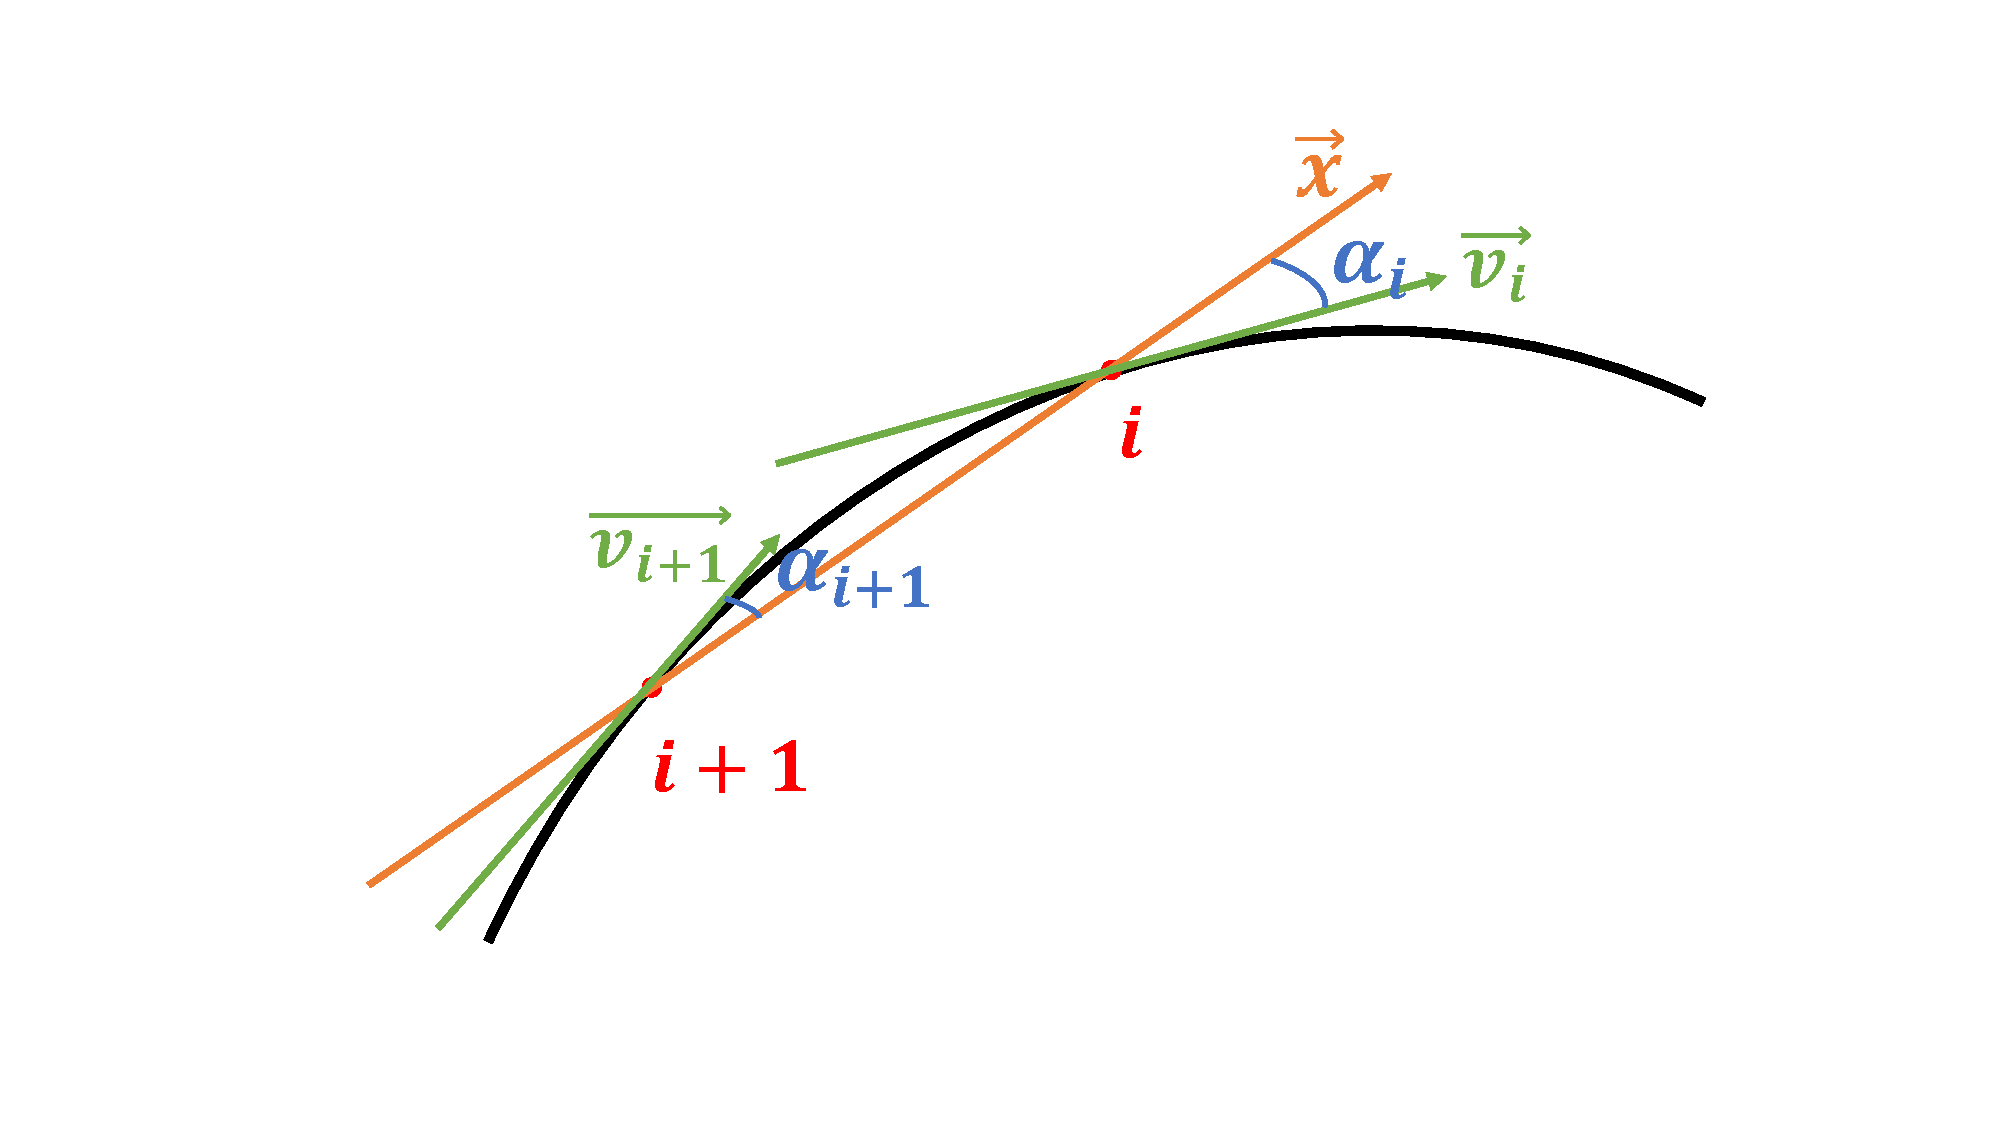
\includegraphics[width=0.6\textwidth]{assets/getv.pdf}
    \caption{\textbf{螺线上两点间关系示意图}}
    \label{螺线上两点间关系示意图}
\end{figure}


\textbf{刚体限制方程}、直角坐标系中的螺线切线方向分别为,
\begin{gather}
    \lvert\vec{v}_{i}\rvert\cos{\alpha_{i}}=\lvert\vec{v}_{i+1}\rvert\cos{\alpha_{i+1}}\mathrm{d}\alpha \\
    \vec{\tau}=-(\cos{\alpha}-\alpha\sin{\alpha}, \sin{\alpha}+\alpha\cos{\alpha}) \label{螺线切线方向}
\end{gather}
又 $\cos{\alpha}=\frac{\lvert\vec{\tau}\cdot\vec{x}\rvert}{\lvert\vec{\tau}\rvert\lvert\vec{x}\rvert}$,代回递推式中得到
\begin{equation}
    \lvert\vec{v}_{i+1}\rvert=\frac{\ \lvert\vec{\tau}_{i+1}\rvert \ \lvert\vec{\tau}_{i}\cdot\vec{x}\rvert\ }{\ \lvert\vec{\tau}_{i}\rvert \ \lvert\vec{\tau}_{i+1}\cdot\vec{x}\rvert\ } \cdot \lvert\vec{v}_{i}\rvert
\end{equation}



题目已经给出了初始条件(龙头的行进速度),即$\lvert\vec{v}_{0}\rvert$,由此只需要计算出每个点的$\vec{\tau}$即可通过递推的方法求得每个点的速度。

\subsubsection{模型求解结果}

计算结果已经保存到\textbf{result1.xlsx}中,这里给出0 s、60 s、120 s、180 s、240 s、300 s时,龙头前把手、龙头后面第 1、51、101、151、201 节、龙身前把手和龙尾后把手的位置和速度,详见表 \ref*{问题1位置结果} 和表 \ref*{问题1速度结果}。

\begin{table}[H]
    \centering\small
    \caption{\textbf{问题1中各时刻板凳龙不同部位所处位置}}
    \label{问题1位置结果}
    \begin{tabular}{|c|c|c|c|c|c|c|}
        \hline
         & 0 s & 60 s & 120 s & 180 s & 240 s & 300 s\\ \hline
        龙头x (m) &8.800000&5.799209&-4.084887&-2.963609&2.594494&4.420274
        \\ \hline
        龙头y (m) &0.000000&-5.771092&-6.304479&6.094780&-5.356743
        &2.320429
        \\ \hline
        第1节龙身x (m) &8.363824&7.456758&-1.445473&-5.237118&4.821221&2.459489\\ \hline
        第1节龙身y (m) &2.826544&-3.440399&-7.405883&4.359627&-3.561949&4.402476\\ \hline
        第51节龙身x (m) &-9.518732&-8.686317&-5.543150&2.890455&5.980011&-6.301346
        \\ \hline
        第51节龙身y (m) &1.341137&2.540108&6.377946&7.249289&-3.827758&0.465829\\ \hline
        第101节龙身x (m) &2.913983&5.687116&5.361939&1.898794&-4.917371&-6.237722\\ \hline
        第101节龙身y (m) &-9.918311&-8.001384&-7.557638&-8.471614&-6.379874&3.936008\\ \hline
        第151节龙身x (m) &10.861726&6.682311&2.388757&1.005154&2.965378&7.040740\\ \hline
        第151节龙身y (m) &1.828753&8.134544&9.727411&9.424751&8.399721&4.393013\\ \hline
        第201节龙身x (m) &4.555102&-6.619664&-10.627211&-9.287720&-7.457151&-7.458662\\ \hline
        第201节龙身y (m) &10.725118&9.025570&1.359847&-4.246673&-6.180726&-5.263384\\ \hline
        龙尾(后)x (m) &-5.305444&7.364557&10.974348&7.383896&3.241051&1.785033\\ \hline
        龙尾(后)y (m) &-10.676584&-8.797992&0.843473&7.492370&9.469336&9.301164\\ \hline
        
    \end{tabular}
\end{table}

\begin{table}[H]
    \centering\small
    \caption{\textbf{问题1中各时刻板凳龙不同部位的速度}}
    \label{问题1速度结果}
    \begin{tabular}{|c|c|c|c|c|c|c|}
        \hline
        & 0 s & 60 s & 120 s & 180 s & 240 s & 300 s\\ \hline
        龙头( $\mathrm{m}\cdot \mathrm{s}^{-1}$) &1.000000&1.000000&1.000000&1.000000&1.000000&1.000000\\ \hline
        第1节龙身( $\mathrm{m}\cdot \mathrm{s}^{-1}$) &0.999971&0.999961&0.999945&0.999917&0.999859&0.999709\\ \hline
        第51节龙身( $\mathrm{m}\cdot \mathrm{s}^{-1}$) &0.999742&0.999662&0.999538&0.999331&0.998941&0.998065\\ \hline
        第101节龙身( $\mathrm{m}\cdot \mathrm{s}^{-1}$) &0.999575&0.999453&0.999269&0.998971&0.998435&0.997302\\ \hline
        第151节龙身( $\mathrm{m}\cdot \mathrm{s}^{-1}$) &0.999448&0.999299&0.999078&0.998727&0.998115&0.996861\\ \hline
        第201节龙身( $\mathrm{m}\cdot \mathrm{s}^{-1}$) &0.999348&0.999180&0.998935&0.998551&0.997894&0.996574\\ \hline
        龙尾(后)( $\mathrm{m}\cdot \mathrm{s}^{-1}$) &0.999311&0.999136&0.998883&0.998489&0.997816&0.996478\\ \hline
    \end{tabular}
\end{table}

\newpage
\subsubsection{部分结果可视化}

盘入螺线和 t=290 s 时板凳龙位置示意图如图 \ref*{部分结果可视化} 所示。

\begin{figure}[H]\centering
\begin{subfigure}[t]{0.47\textwidth}\centering
    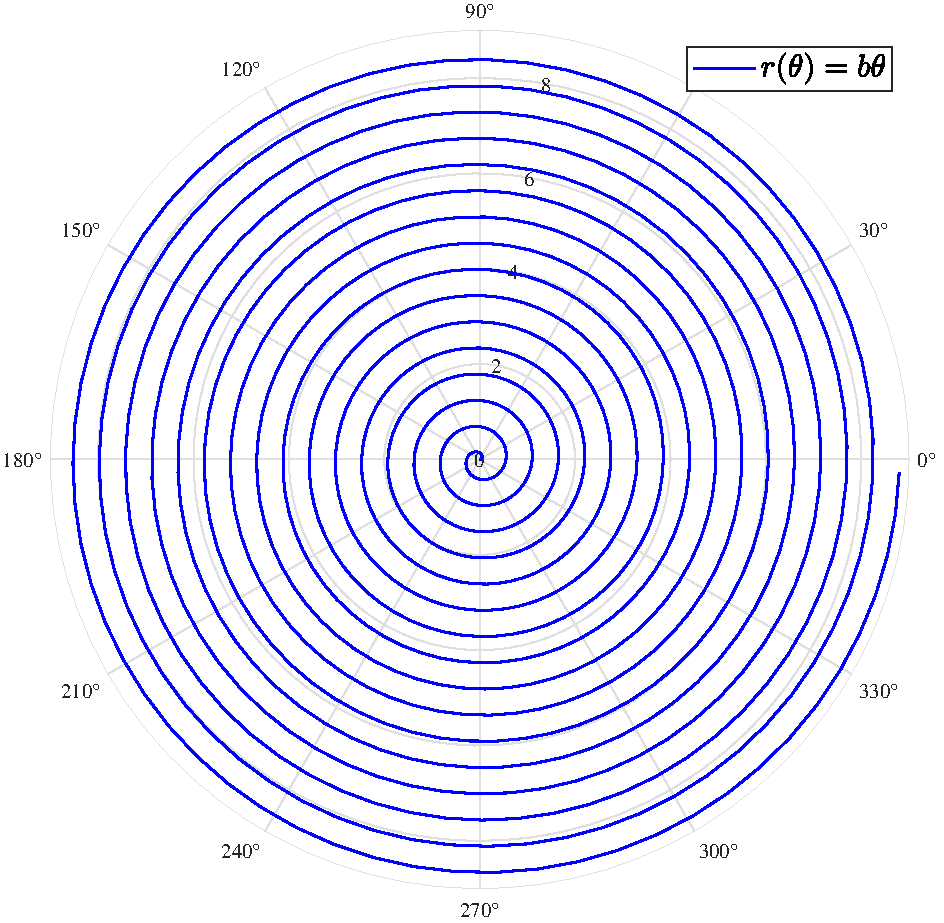
\includegraphics[width=0.95\textwidth]{assets/ajmd.pdf}
    \caption{\bfseries 阿基米德螺线示意图 }
\end{subfigure}\begin{subfigure}[t]{0.47\textwidth}\centering
    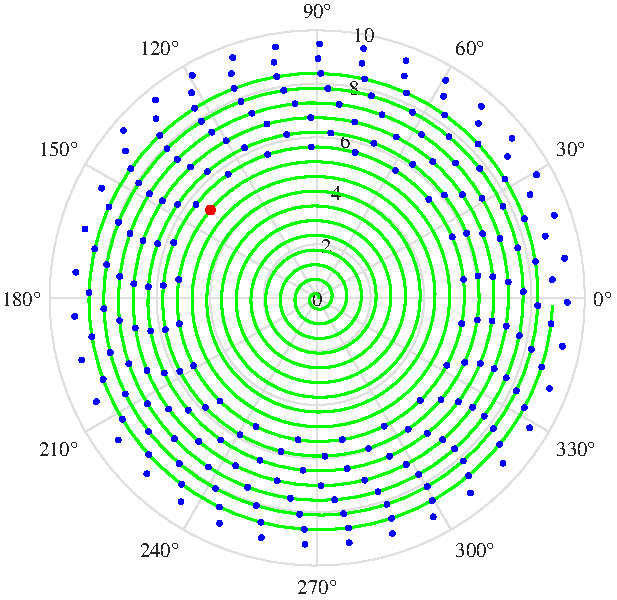
\includegraphics[width=0.95\textwidth]{assets/t1circle.pdf}
    \caption{\bfseries t = 290 s 时板凳龙全把手位置示意图 }
\end{subfigure}
\caption{\bfseries 部分结果可视化 }\label{部分结果可视化}
\end{figure}


\subsection{问题二}
\subsubsection{舞龙队碰撞检测模型模型}
对于问题二,我们可以根据问题一的做法,得到每一对把手的位置信息,而每一对相邻把手可以定位一张板凳。所以,考虑每一对相邻把手,我们向外扩展出一个矩形,最终的扩展结果即为板凳龙的俯视效果。通过矩形顶点的位置关系,可以判断板凳间是否存在重叠情况,进而得知是否发生碰撞。

撞击过程如图所示:

\begin{figure}[H]\centering
\begin{subfigure}[t]{0.47\textwidth}\centering
    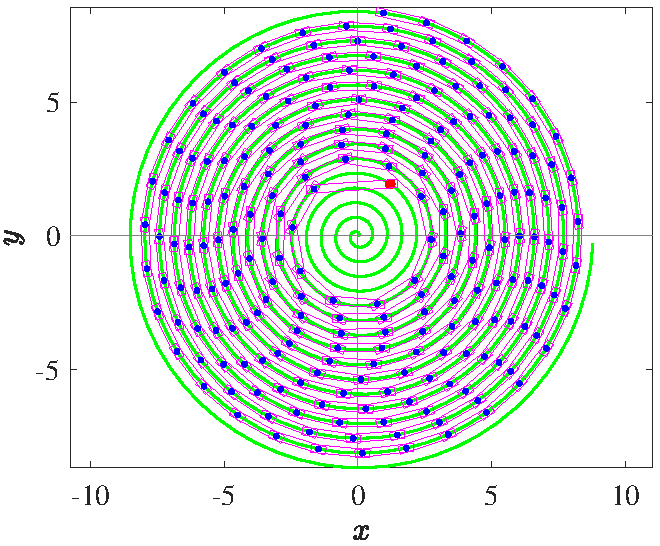
\includegraphics[width=0.95\textwidth]{assets/Q2碰撞示意图.pdf}
    \caption{\bfseries 碰撞瞬间舞龙队位置 }
\end{subfigure}\begin{subfigure}[t]{0.47\textwidth}\centering
    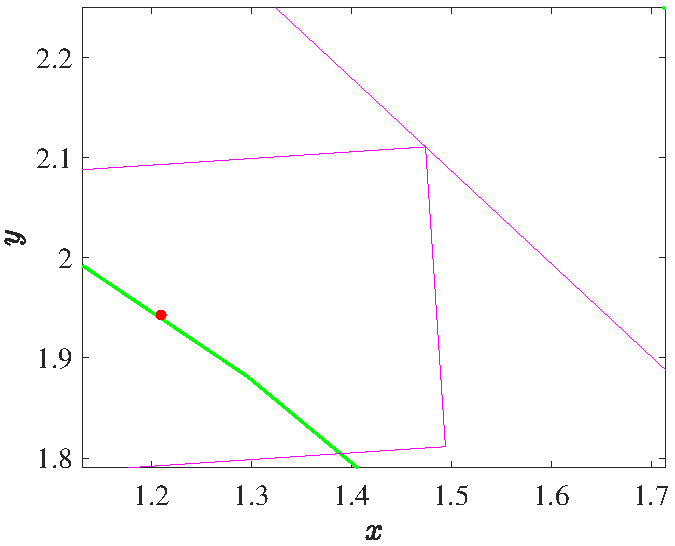
\includegraphics[width=0.95\textwidth]{assets/Q2碰撞示意图(放大).pdf}
    \caption{\bfseries 碰撞点局部放大 }
\end{subfigure}
\caption{\bfseries 撞击过程 }
\end{figure}

我们可以进一步优化对于碰撞过程的判定。因为除龙头外所有的板凳完全一致,所以第三块和后续所有板凳一定会\textbf{重复第二块板凳的运动},因此我们只需要考虑第一、二块板凳是否会与其他板凳发生碰撞。又因为第一、二块板凳的内圈不存在其他板凳,不需要考虑。所以最终我们只需要定位第一、二块板凳\textbf{外侧的两个顶点},共计四个点是否在其他矩形内即可判断是否发生碰撞。

判断是否发生碰撞的具体方法推导如下:如图所示,下方的板凳为龙头或第二块板凳(余下的无需考虑),以 $i$ 号板凳(对应 $i$ 号把手和 $i+1$ 号把手)的 1 号点为新坐标系的原点,以 $\vec{v}_{i,1}$ 和 $\vec{v}_{i,2}$ 为基底,建立新直角坐标系 $O'$。记 $\vec{p}_{i,k} = ({p}_{i,k,x},\ {p}_{i,k,y})$ 为第 $i$ 号板凳的 $k$ 号顶点坐标,则有 
\begin{gather}
    \vec{v}_{i,1}=\vec{p}_{i,2}-\vec{p}_{i,1}=(p_{i,2,x}-p_{i,1,x}\enspace,\enspace p_{i,2,y}-p_{i,1,y})\\
    \vec{v}_{i,2}=\vec{p}_{i,4}-\vec{p}_{i,1}=(p_{i,4,x}-p_{i,1,x}\enspace ,\enspace p_{i,4,y}-p_{i,1,y})
\end{gather}
\begin{figure}[H]
    \centering
    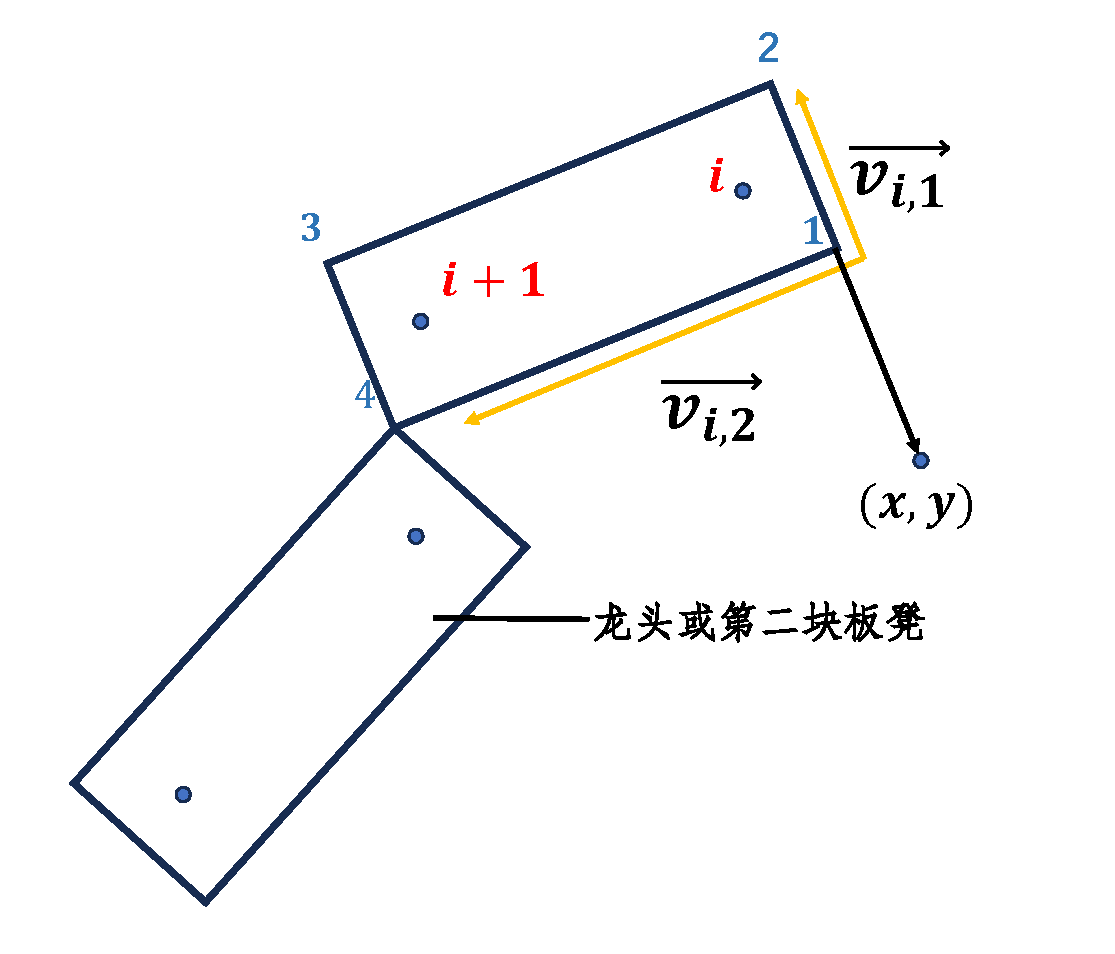
\includegraphics[width=0.43\textwidth]{assets/t2crush.pdf}
    \caption{\textbf{发生碰撞的情形示意图}}
    \label{发生碰撞的情形示意图}
\end{figure}

接下来进行坐标系的转换。在线性空间 $V$ 中,设 $\vec{x} = (x, y) \in \R^2,\ v = \vec{x}\cdot\vec{v}_0$,其中 $\vec{v}_0$ 为 $V$ 的一组基,则对于任意的线性映射 $\varphi$,我们有:
\begin{equation}
\varphi(v) = \vec{x}A_\varphi\vec{v}_0
\end{equation}
代入本题,得到坐标系变换公式:
\begin{equation}
\vec{x}'= (a,b) = (\vec{x} - \vec{x}_O)A_\varphi^{-1}
\end{equation}
其中 $\vec{x}'$ 表示在新坐标系 $O$ 下的位置向量,转换矩阵 $A_\varphi$ 为
\begin{equation}
A_\varphi =     
\begin{bmatrix} 
    p_{i,2,x}-p_{i,1,x} & p_{i,2,y}-p_{i,1,y}\\ 
    p_{i,4,x}-p_{i,1,x} & p_{i,4,y}-p_{i,1,y}\\ 
\end{bmatrix}
\end{equation}

至此上式,可以解出转坐标系后的新一组坐标 $(a,b)$。若$a\in(0,1)$且$b\in(0,1)$则发生碰撞,否则未发生碰撞。

当判断完成后我们还需要进一步考虑如何得到精确的碰撞时间,考虑使用\textbf{变步长迭代法},对时间 $t$ 进行迭代。

\textbf{变步长迭代法实现流程如下:}第一次迭代为粗测,迭代步长较长。将时间步长设置的稍大一些,在第一次发现碰撞情况后停止。由于步长较大,可能出现漏测情况,所以将时间向前回调十个步长,并可认为这一时间内范围内发生了第一次碰撞。

接下来,调小时间步长,在缩小的时间范围上进行二次迭代,将第一次碰撞的时间锁定在较精确的区间内,以确保没有漏过某次碰撞,且此区间不会出现其它碰撞情况。

最后利用\textbf{二分法},下界 $\text{bound}_\text{low}$ 为最早的未碰撞时间,上界 $\text{bound}_\text{up}$ 为最晚的已碰撞时间,不断二分时间,并判断当前时刻是否发生碰撞,以此提高精度。

\subsubsection{模型求解结果}

求解上述模型,得到:
\begin{equation}
\text{ \textbf{碰撞时间} $t_{crushed} = $ \textbf{412.473838s}}
\end{equation}

其它计算结果详见文件 \textbf{result2.xlsx}。

\subsection{问题三:}

问题三和问题二的\textbf{本质是相同的}。只需要改变螺距,再通过问题二中的模型计算出碰撞时对应的半径(后称为碰撞半径)。若碰撞半径小于调头半径(龙头在调头区内),则符合题目条件,可以将螺距进一步缩小,否则不符合题目条件,需要调大螺距。

考虑到所有板凳的宽度为 0.3 m,螺距的大小不应小于 0.35 m。在实际计算螺距时,我们有\textbf{两种不同的思路},下面依次说明。

\subsubsection{思路一:基于二分法的最小螺距求解模型}

作出 螺距大小(横坐标)与碰撞半径(纵坐标)之间的关系图,如图 \ref*{螺距范围 [0.35 m, 0.55 m]} 和图 \ref*{螺距范围 [0.44 m, 0.46 m]} 所示。由图可知,在调头半径附近,碰撞半径和螺距大小是\textbf{严格单调}的,因此很自然地考虑到,利用\textbf{二分法}对制定螺距范围进行二分,并得到精度优秀的结果。

\begin{figure}[H]\centering
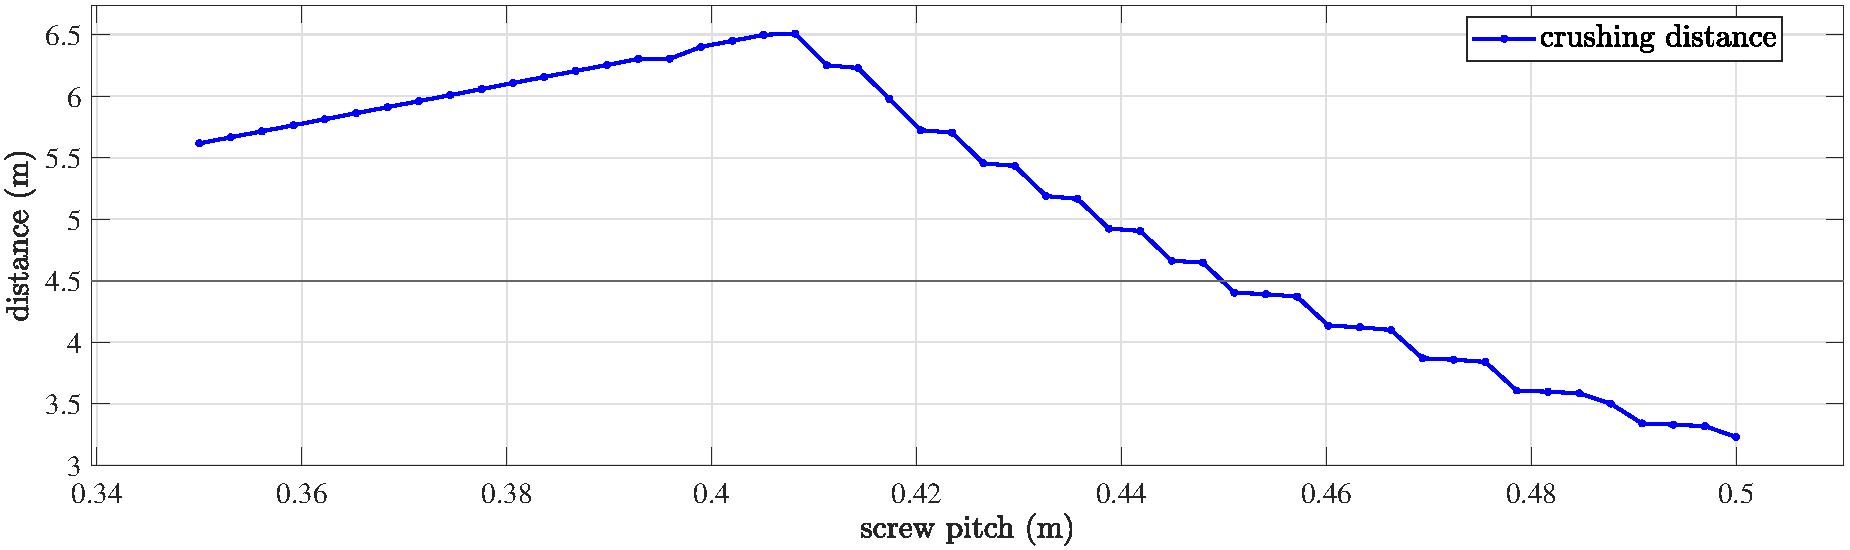
\includegraphics[width=\textwidth]{assets/Q3大范围.pdf}
\caption{\bfseries 螺距范围 [0.35 m, 0.55 m] }\label{螺距范围 [0.35 m, 0.55 m]}
\end{figure}
\begin{figure}[H]\centering
    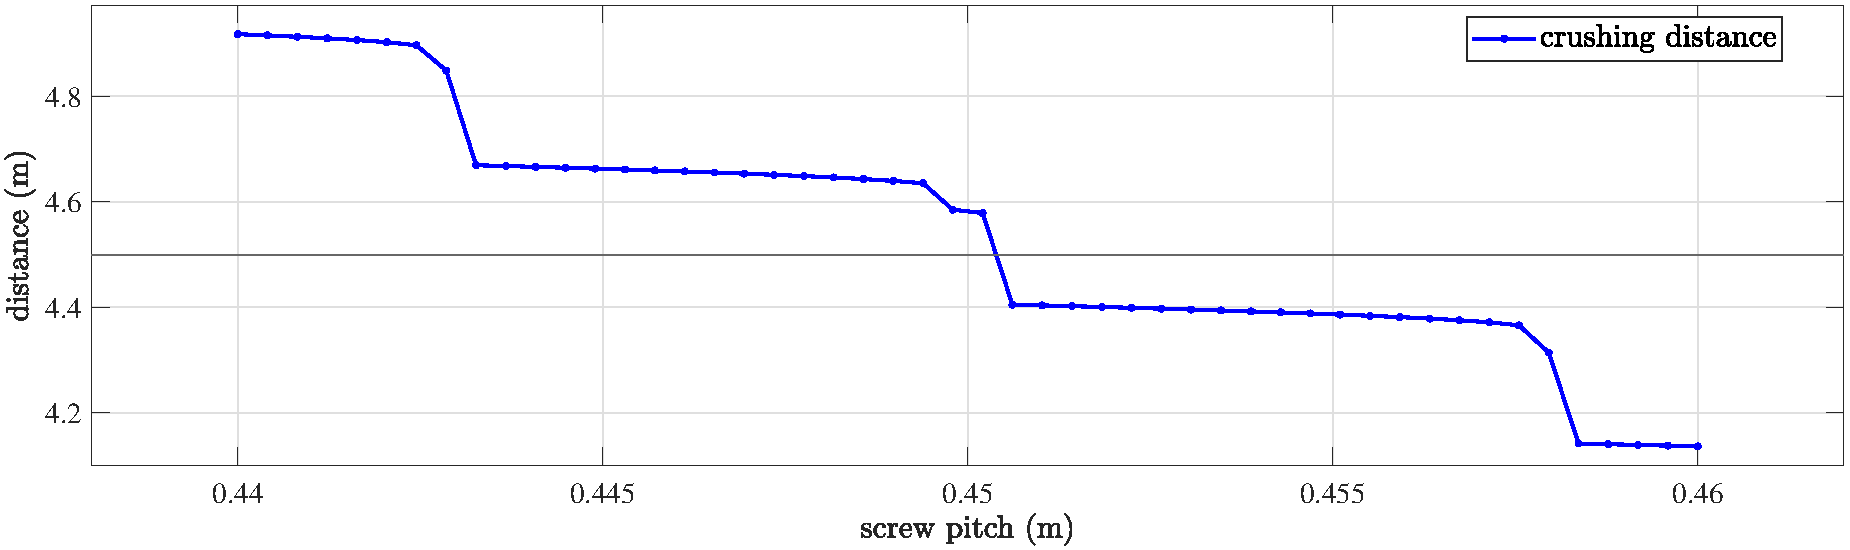
\includegraphics[width=\textwidth]{assets/Q3小范围.pdf}
    \caption{\bfseries 螺距范围 [0.44 m, 0.46 m]}\label{螺距范围 [0.44 m, 0.46 m]}
    \end{figure}

\subsubsection{思路二:基于模拟退火的最小螺距求解模型}

\textbf{模拟退火算法}是基于蒙特卡洛迭代求解策略的一种\textbf{随机寻优算法},该算法在搜索过程中引入随机变量,并以一定概率接受一个比当前解差的解,因此可以有效避免陷入局部最优解,找到\textbf{全局最优解}。

在本题中,我们的具体求解步骤如下:
\begin{enumerate}[leftmargin=4.5em]
\item 初始化参数:
设置退火初始温度$T_{0}=50\ ^\circ$C,温度下降系数$\alpha=0.98$,结束温度$T_{end}=0.1\ ^\circ$C,马尔科夫链长度$L_{\text{mkv}}=6$。仅有一个参数(螺距),参数范围为 $[0.35\ \mathrm{m}, 0.5\ \mathrm{m}]$。

\item 生成新解:
根据当前最优解,在合理范围下生成一定的扰动,并生成新解$\vec{x}$。

\item 检验新解:根据生成的新解,计算目标函数增量 $\Delta{E}$,若满足$\Delta{E}<0$,则接受新解,否则计算接受新解的概率,判断是否接受新解,并进行降温。
\item 结束退火:若当前温度达到终止温度 $T_{end}$,输出最终结果,结束退火过程。
\end{enumerate}
\vspace*{1em}
模拟退火流程图如下:

\begin{figure}[H]
    \centering
    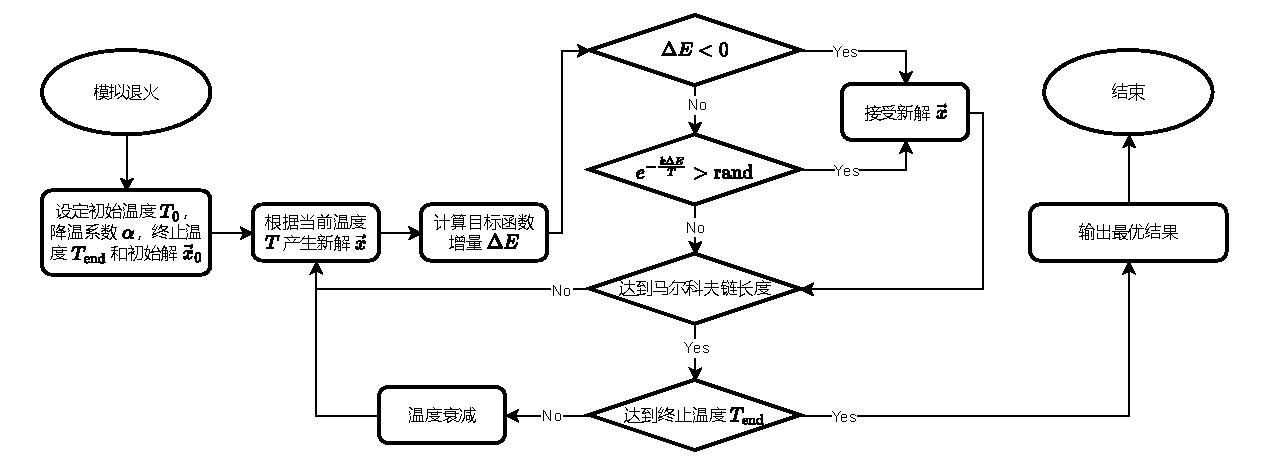
\includegraphics[width=0.9\textwidth]{assets/simulate_process.pdf}
    \caption{\textbf{模拟退火流程图}}
    \label{模拟退火流程图}
\end{figure}


此外,我们还可以进行多次模拟,且尝试选择偏离正常螺距较大的数值作为起点进行模拟后,将得到的数据进行对比,分析结果的稳定性和收敛性。

\subsubsection{模型求解结果}

两种方法得到的最小螺距结果为:
\begin{equation}
\text{\textbf{二分法最小螺距: 0.450337 m},\textbf{模拟退火最小螺距: 0.450297 m}}
\end{equation}

结果之间的\textbf{绝对误差为 0.008882 \%}。两相对照之下可以认为两种做法均可行,得到的\textbf{结果合理且有较高精度}。

%\begin{table}[H]
%    \centering
%    \caption{\textbf{最小螺距求解结果}}
%    \label{最小螺距求解结果}
%    \begin{tabular}{|c|c|}
%        \hline
%        二分法 & 模拟退火\\
%        \hline
%        0.450337 m& 0.450297 m\\
%        \hline
%    \end{tabular}
%\end{table}

实际运行时的模拟退火过程如下,由退火过程图可知,模拟退火结果收敛性较好,且有较高精度。

\begin{figure}[H]
    \centering
    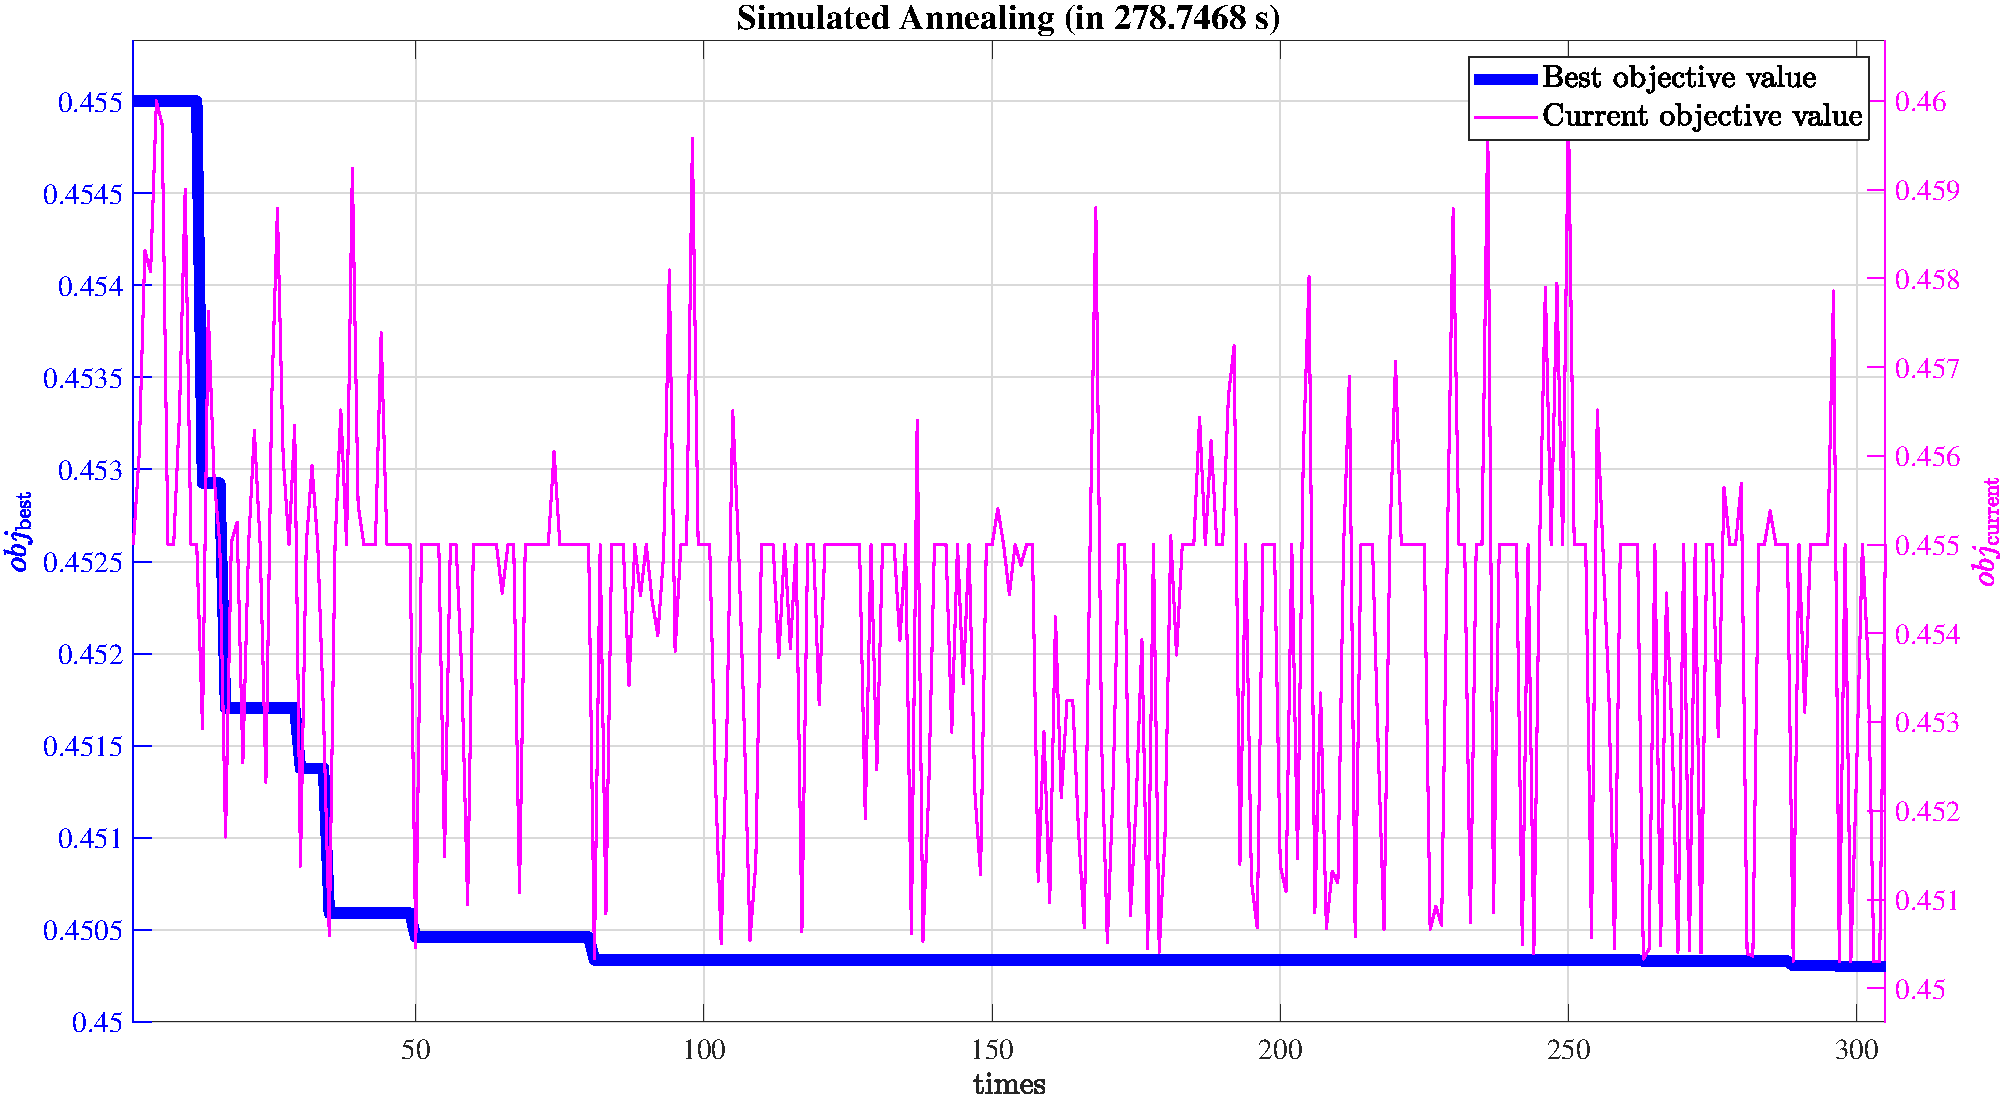
\includegraphics[width=0.86\textwidth]{assets/模拟退火过程.pdf}
    \caption{\textbf{模拟退火过程}}
    \label{模拟退火过程}
\end{figure}

%\subsubsection{部分结果可视化}
%
%在最小螺距下,分别作出 t=10 s 和 t=290 s 时板凳龙俯视图,可见龙头在%调头区内时,龙头半径和碰撞半径的关系。
%
%\begin{figure}[H]
%    \begin{minipage}{0.49\linewidth}
%        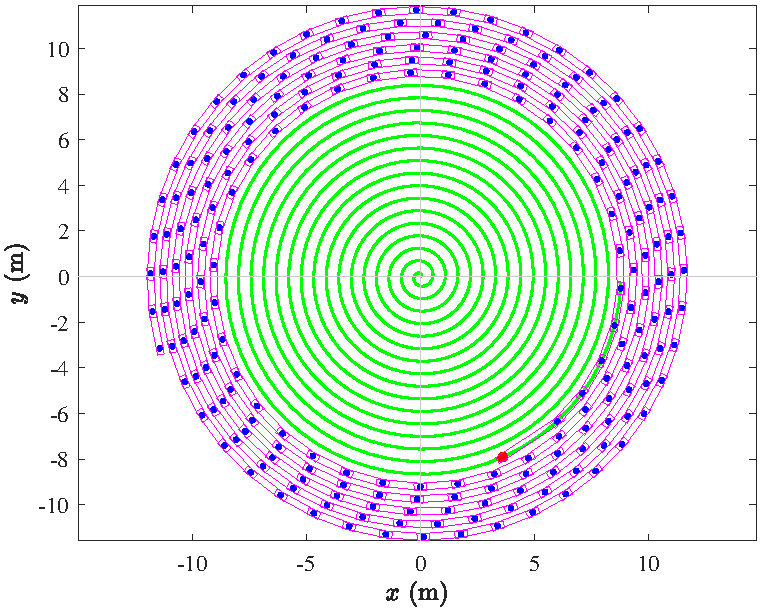
\includegraphics[width=1.0\textwidth]{assets/t2circle2.%pdf}
%        \caption{t=10 s时板凳龙俯视图}
%        \label{FIG:1}
%    \end{minipage}
%    \begin{minipage}{0.49\linewidth}
%        \includegraphics[width=1.0\textwidth]{assets/%create_square.pdf}
%        \caption{t=290 s时板凳龙俯视图}
%        \label{FIG:1}
%    \end{minipage}
%\end{figure}



\subsection{问题四:}

\subsubsection{实际调头路径的几何性质}

问题四可分为两部分,一部分是求解最优调头位置,另一部分是根据实际调头路径,求解位置和速度结果。

对于前半部分,考虑到板凳龙进入调头空间后\textbf{不一定马上开始调头},而是可以继续沿着螺线前进。为了确定这一情况下的最短调头曲线,我们需要研究调头曲线的几何性质。我们注意到,实际调头路径的起始点和中止点可以不中心对称,这样会导致全路径曲线的参数方程求解困难。为了保持计算精度的同时,尽可能地简便计算,我们在后续问题中,\textbf{规定调头路径的起始点和中止点中心对称}。

在规定了中心对称后,可以得到如下结论:板凳龙进入调头区域后,\textbf{沿螺线走的越远(越晚开始调头),调头曲线长度就越短}。为了证明这一结论,首先要证明:调头曲线\textbf{形状唯一},并且,其长度只与实际调头起始点的半径长(与原点距离)有关,只会随开始调头时间等比缩放。

\textbf{具体证明如下:}

如图 \ref*{调头区域示意图} 所示,点 $M$ 为盘入螺线与实际调头空间的交点,又因为盘出螺线与盘入螺线\textbf{中心对称},所以点 $H$ 为盘出点。作出螺线上点 $H$ 处的切线,与圆交于点 $E$,点 $M$ 处的切线,与圆交于点 $F$,由中心对称可知\textbf{两直线平行},且四边形 $HDMF$ 构成矩形。

因为调头路径与盘入、盘出螺线\textbf{均相切},所以调头路径前后两段圆弧所在的圆一定和$HD$、$MF$\textbf{分别相切}。进而得到两段圆弧所在圆的圆心(设前半段为圆弧圆心为$C$、后半段圆弧圆心为$A$)一定分别位于直线$MD$、$HF$上。

\begin{figure}[H]
    \centering
    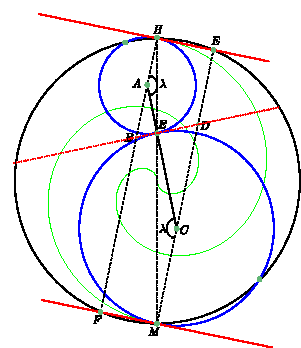
\includegraphics[width=0.4\textwidth]{assets/t4circle.pdf}
    \caption{\textbf{调头区域示意图}}
    \label{调头区域示意图}
\end{figure}

由题目条件可知,两段圆弧所在的圆是相切的,设切点为$E$,则有$AE$、$CE$均垂直于图中红色虚线$BD$,所以$A$、$E$、$C$\textbf{三点共线}。因为$MD$平行于$HF$,所以$\angle{HAC}=\angle{MCA}$。由题目条件可知两圆的半径比为 2:1。又有两个圆心角$\angle{HAC}=\angle{MCA}$相等,所以可知,$ME:EH=2:1$,因此,点$E$可以被唯一确定。由此两个圆\textbf{是唯一确定的},所以整条调头路径\textbf{是唯一确定的},所以整条调头曲线的长度只会守两个圆的半径影响,而两圆的半径又能被调头区域的直径\textbf{唯一确定},因此调头曲线的长度\textbf{仅取决于调头起始点与圆心连线的长度}。

又由题目可知两段圆弧的长度比为$\overset{\frown}{ME}:\overset{\frown}{EH}=2:1$,而两端弧的圆心角相等,所以可以推出两个圆的\textbf{半径长度比也为$2:1$}。

考虑到半径长为$2:1$,圆心角相同,所以$ME:EH=2:1$,因此 E 点可以\textbf{被唯一确定},由此两个圆\textbf{是唯一确定的},所以整条调头路径\textbf{是唯一确定的},所以整条调头曲线的长度只会守两个圆的半径影响,而两圆的半径又能被调头区域的直径\textbf{唯一确定},因此调头曲线的长度\textbf{仅取决于调头起始点与圆心连线的长度}。\textbf{证毕}。






\vspace{4mm}

通过上述证明,我们知道:想要得到最短的调头路径,需要在\textbf{“不违法”}的情况下尽可能晚的开始调头。
这里的“违法”有两种情况:

\begin{enumerate}
\item \textbf{发生碰撞}。即在最新路径上板凳龙在行进过程中会发生板凳间的碰撞。
\item \textbf{违背刚体限制}。当某一个板凳在运动过程中,出现了板凳头尾速度向量点乘该板凳本身的速度向量的两个结果异号,这意味着下一瞬间,两节点间的距离会被拉长,也即板凳上的节点长度发生变化,违背了刚体性质。
\end{enumerate}

\subsubsection{求解全路径参数方程}

但在开始迭代前,需要先解出两个圆的方程,以得到调头路径,才能进行进一步编写代码。所以,这里给出\textbf{曲线中两个圆的参数方程}的推导过程。

\begin{figure}[H]
    \centering
    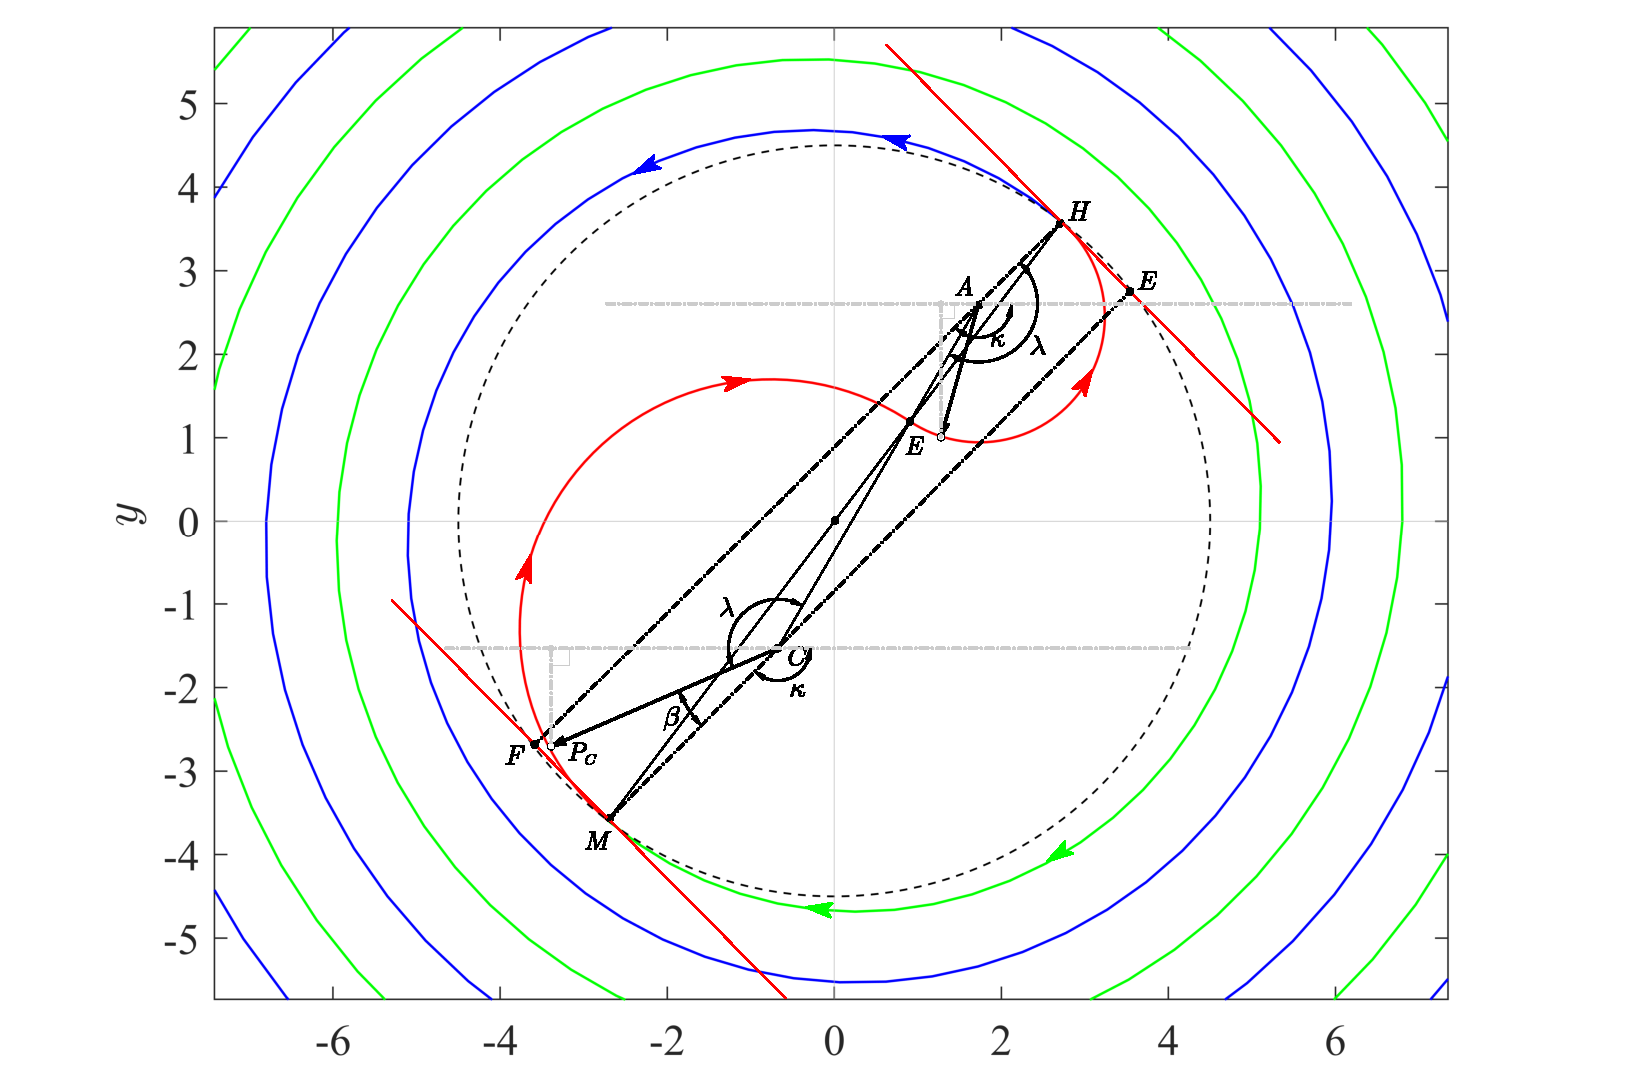
\includegraphics[width=1.0\textwidth]{assets/t4getfunc.pdf}
    \caption{\textbf{调头路径参数方程求解}}
    \label{调头路径参数方程求解}
\end{figure}

如图 \ref*{调头路径参数方程求解} 所示,对于给定的 $r_t$,可根据阿基米德螺线方程 $r=b\theta$ 得到 $\theta_{t}=\frac{r_t}{b}$。点$M$为调头起始点,则有 $M=(b\theta_t\cos{\theta_t},b\theta_t\sin{\theta_t})$,又盘入盘出螺线中心对称,所以点$H$的坐标为 $H=(-b\theta_t\cos{\theta_t},-b\theta_t\sin{\theta_t})$。由先前证明可知,$ME:EH=2:1$,于是 $HE=\frac{1}{3}r_t$,
所以有$OE=\frac{1}{2}EH=\frac{1}{3}HE$,即点E的坐标为 $E=(-\frac{1}{3}x_M, -\frac{1}{3}y_M)$。分别记点 $M$ 处、点 $H$ 处的(螺线)切线方向为 $\vec{l}_M,\ \vec{l}_H$(沿前进方向),则有:
\begin{gather}
    \vec{l}_M=-[\cos{(\theta_t)}-\theta_t\sin{(\theta_t)},\enspace \sin{(\theta_t)}+\theta_t\cos{(\theta_t)}] \\ 
    \vec{l}_H=[\cos{(\theta_t)}-\theta_t\sin{(\theta_t)},\enspace \sin{(\theta_t)}+\theta_t\cos{(\theta_t)}]
\end{gather}

可求得$\overrightarrow{HA}$的方向为:
\begin{equation}
    \vec{l}_{HA}=[0,0,1]\times[\vec{l}_H,0]=(x_{HA}, y_{HA}, 0)
\end{equation}

进而得角 $\kappa$ 的大小 $ \kappa=\pi-\arctan{\frac{y_{HA}}{x_{HA}}}$。
实际计算过程中因为 $\arctan$ 的值域范围是 $[-\frac{\pi}{2},\ \frac{\pi}{2}]$,而 $\kappa$ 的范围是 $[0,\  2\pi]$,两者含义不符,因此除了需要减去 $\pi$,还需要判断 $x_{HA}$ 的正负,并对 $x_{HA} < 0$ 时的 $\kappa$ 进行修正,才能得到计算所需要的正确 $\kappa$ 的值。具体而言,我们有:
\begin{equation}
\kappa = 
\begin{cases}
    \pi-\arctan{\frac{y_{HA}}{x_{HA}}}, & x_{HA} \leqslant 0 \\
    -\arctan{\frac{y_{HA}}{x_{HA}}}, & x_{HA}>0 \\
\end{cases}
\end{equation}

考虑用 $A = (x_A, y_A)$ 表示点 A 的坐标,$H = (x_H, y_H)$ 表示点 E 的坐标,以此类推。设点 $A$ 为:
\begin{equation}
    A=H+n\cdot\vec{l}_{HA} \Longrightarrow 
    \begin{cases}
        x_A=x_H+n\cdot x_{HA}\\
        y_A=y_H+n\cdot y_{HA}
    \end{cases}
\end{equation}

其中$n$为待定未知量。根据半径相等,又有方程:
\begin{equation}
| \overrightarrow{AE} | = | \overrightarrow{AH} | \Longrightarrow  f(n) = \lvert E-A\rvert-\lvert H-A\rvert\notag=0
\end{equation}

解此方程,得到 $n$ 的值,也即求出了点$A$的坐标。又$\vec{OC}=\vec{OA}+3\vec{AE}$,所以点$C$的坐标为 $C = 3E - 2A$,至此,两个圆心的坐标都已确定。

对于角度 $\lambda$,在小圆中由余弦定理可得:
\begin{equation}
\lambda = \arccos{(1-\frac{| \overrightarrow{HE} |^{2}}{2 | \overrightarrow{AH} | ^{2}})}
\end{equation}

设原坐标系 $O$ 的基向量为 $\vec{e}_1=(1,0)$、$\vec{e}_2=(0,1)$,大圆的半径为$R_1$,小圆的半径为$R_2$,可以求得圆 $C$ 的参数方程:
\begin{gather}
P_C  = C + \overrightarrow{CP} = C + R\cos(\beta + \kappa)\vec{e}_1 - R_1\sin(\beta + \kappa)\vec{e}_2  \\ 
\Longleftrightarrow 
\begin{cases}
    x = x_C + R_1\cdot\cos{(\beta+\kappa)}\\
    y = y_C - R_1\cdot\sin{(\beta+\kappa)}
\end{cases}
\end{gather}

在圆 $C$ 中$\beta$ 的正方向是顺时针,而在圆 $A$ 中$\beta$ 的正方向是逆时针,因此结合角度关系后,作映射 $\beta \longmapsto -\beta$,得到圆 $A$ 的参数方程为:
\begin{gather}
P_A = A + \overrightarrow{AP} = A - R_2\cos{(-\beta+\kappa+\lambda)}\vec{e}_1 + R_2\sin{(-\beta+\kappa+\lambda)}\vec{e}_2 \\
\Longleftrightarrow     
\begin{cases}
    x = x_A - R_2\cdot\cos{(-\beta+\kappa+\lambda)}\\
    y = y_A + R_2\cdot\sin{(-\beta+\kappa+\lambda)}
\end{cases}
\end{gather}




至此我们就计算出了两个圆的参数方程,后续每一步迭代过程中都需要求出最新的调头路径,以判断是否发生碰撞,或是否存在某一时刻出现速度“违法”,即违背了刚体限制的情况(同一板凳的头尾速度向量分别点乘该板凳本身的速度向量,若两个结果异号,则破坏刚体限制)。

\subsubsection{最小实际调头半径模型建立}

基于上述理论,我们考虑最晚在什么时刻开始调头是合法的,这一问题与问题 2 不谋而合,我们仍用变步长搜索法结合二分法来解决。考虑对实际调头半径 $r_{t}$ 进行迭代,对于每一个 $r_{t}$,计算新的行进路线上是否出现“违法情况”,并逐步调整实际调头半径,经过变步长搜索后,得到较精确调头半径范围,再利用二分法得到高精度结果。

\subsubsection{最小实际调头半径求解结果}

求解上述模型,得到:
\begin{equation}
\text{\textbf{最小实际调头半径为} $r_t=$ \textbf{4.254674 m}}
\end{equation}

由此可以得到板凳龙从\textbf{盘入、调头到盘出}的全过程路径图,如图 \ref*{板凳龙路径示意图} 所示。其中,图 \ref*{板凳龙路径示意图} (b) 中的黑色虚线表示题目中给出的调头区域范围,红色虚线表示实际调头区域范围。
\begin{figure}[H]\centering
\begin{subfigure}[t]{0.48\textwidth}\centering
    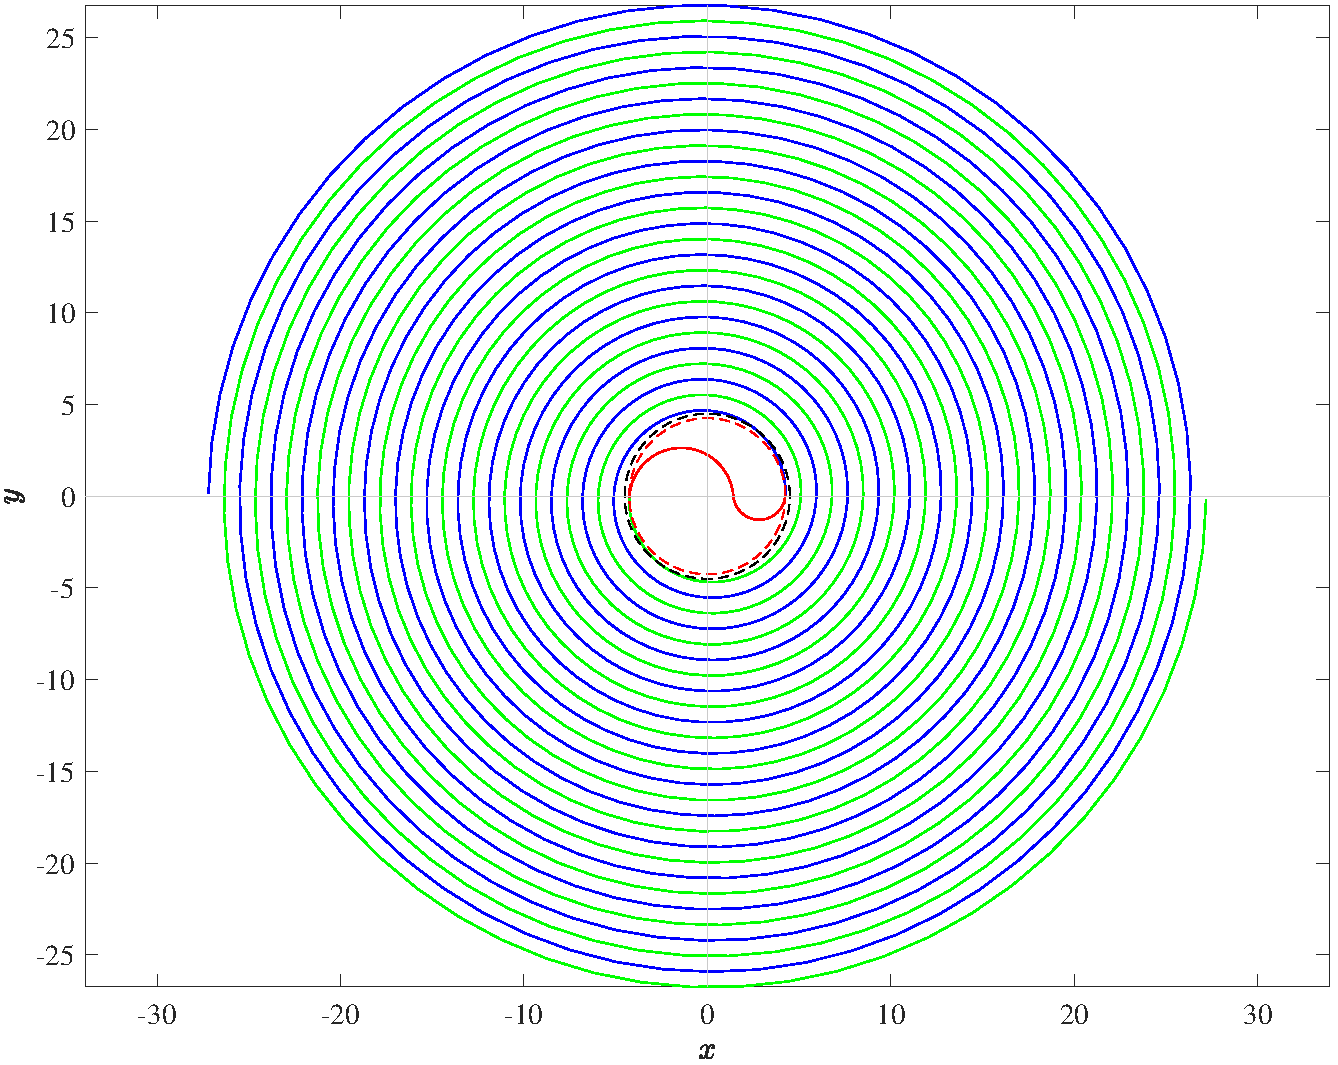
\includegraphics[width=\textwidth]{assets/Q4全路径.pdf}
    \caption{\bfseries 全路径曲线(盘入、调头、盘出) }
\end{subfigure}\begin{subfigure}[t]{0.48\textwidth}\centering
    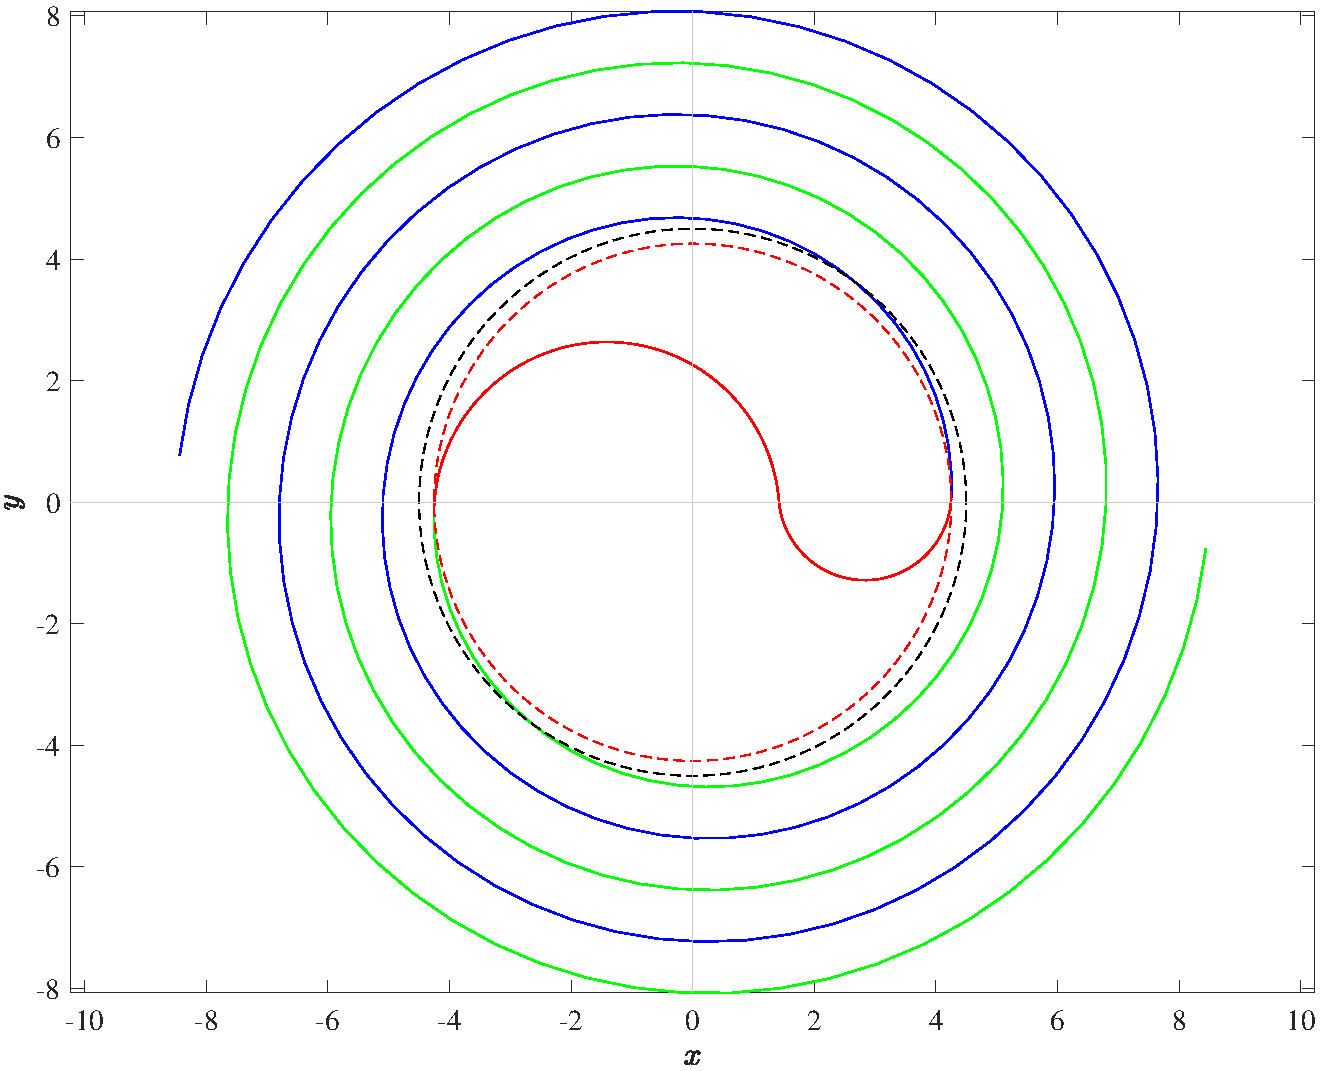
\includegraphics[width=\textwidth]{assets/Q4实际调头位置.pdf}
    \caption{\bfseries 调头空间与实际调头位置 }
\end{subfigure}
\caption{\bfseries 板凳龙路径示意图 }\label{板凳龙路径示意图}
\end{figure}

\subsubsection{全路径位置速度模型建立}

对于要求计算的数据,其中 [-100 s, 0 s) 部分,板凳龙还在盘入螺线上,这部分计算方式和问题一是完全相同的。而对于 [0 s, 100 s] 的部分,需要根据全路径参数方程计算出各把手的位置和速度。

在实际实现过程中,还需要注意判断当前把手所处的曲线为哪一段(盘入、调头、盘出)。所处位置不同,计算速度时需要的切线方向(速度方向)也不同。

盘入和盘出螺线上的节点的切线方向仍由式 \ref*{螺线切线方向} 给出,圆弧上的节点的切线方向由下式给出:
\begin{gather}
\vec{\tau} = (x_{\tau},y_{\tau}, 0) = 
\begin{cases}
    - [0, 0 , 1] \times \overrightarrow{CP},\quad & \text{点 P 位于大圆弧} \\
    [0, 0 , 1] \times \overrightarrow{AP},\quad & \text{点 P 位于小圆弧} \\
\end{cases}
\end{gather}

由此可以计算任意时刻下的舞龙队位置和速度。

\subsubsection{问题四后半部分求解结果}

设定极角求解精度为 $10^{-16}$ 进行求解,最终计算结果存放在\textbf{result4.xlsx}中。

图 \ref*{100 s 时板凳龙各把手位置示意图} 为 $t$ = 100 s 时,板凳龙各把手的位置结果可视化,其中粉色圆点表示龙头。

\begin{figure}[H]
    \centering
    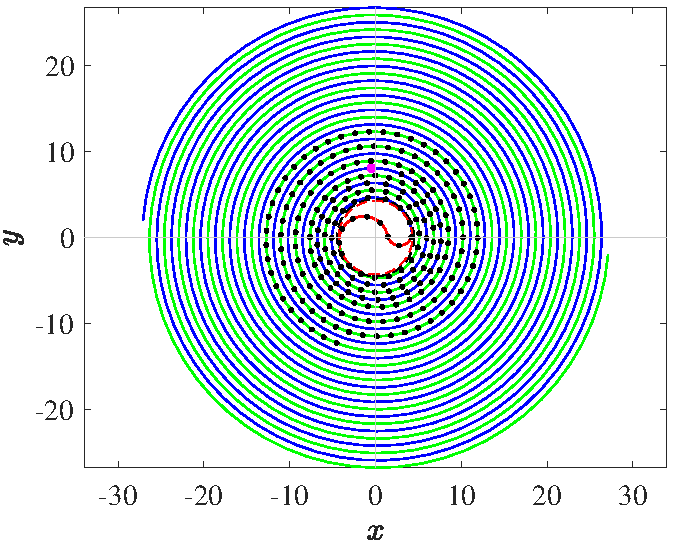
\includegraphics[width=0.65\textwidth]{assets/t4circle_100.pdf}
    \caption{\textbf{100 s 时板凳龙各把手位置示意图}}
    \label{100 s 时板凳龙各把手位置示意图}
\end{figure}


\subsection{问题五}

\subsubsection{龙头最大速度迭代模型}

问题五回归到第一问,仅需考虑每个把手的位置和速度。

易见龙头的速度范围是 [0 $\mathrm{m\cdot s^{-1}}$, 2 $\mathrm{m\cdot s^{-1}}$] ,考虑将龙头的行进速度直接设定为最大值 2 $\mathrm{m\cdot s^{-1}}$,根据问题一中的递推结论,由龙头速度可以递推得到每个把手的速度。设定合适的时间步长,模拟舞龙队的前行过程,若某一时刻发现存在一个把手的速度大于 2 $\mathrm{m\cdot s^{-1}}$,则考虑将龙头的速度降低,使当前出现错误的把手此刻的速度正好等于 2 $\mathrm{m\cdot s^{-1}}$。这与从一开始龙头的速度就被降低是一致的,因为行进路径不变,速度满足刚体限制(递推关系),各节点间的速度应是等比缩放的。

对于板凳龙的模拟行进长度,由于调头区域的两个圆的\textbf{曲率}明显大于阿基米德螺线上的点的曲率,且在进入盘出螺线后,根据问题一对速率的计算结果,越向螺线外圈行进,速度越趋近龙头速度,所以最终需要模拟的前行范围,是从板凳龙进入调头区域开始,直到板凳龙完整通过调头路径曲线为止。

后续不断重复上述过程,直到所有把手在任何时刻的最大速度都不超过 2 $\mathrm{m\cdot s^{-1}}$,即可得到龙头的最大行进速度。

\subsubsection{问题五模型求解结果}

设定求解时间步长为 $10^{-7}$ s,经计算,\textbf{龙头的最大行进速度为:}
\begin{equation}
\text{\textbf{$v_{max}=$ 0.409122 $\mathbf{m}\cdot \mathbf{s^{-1}}$}}
\end{equation}

\section{模型评价与推广}
\subsection{模型优点}

\subsubsection{优点一:}
本文的建模始终基于数学理性思维,利用刚体物理、平面几何、线性代数等数学理论建立模型,结合现实经验进行优化,对多个结论进行了可靠性分析或结果可视化。模型的构建基于清晰的物理意义和数学表达,便于其他研究者理解和实现,有利于学术交流和技术传播。模型建立、结果分析较为严谨、全面。
\subsubsection{优点二:}
本文在对问题三的求解过程中应用了模拟退火启发式算法和二分法,同时推进,互相验证,保证了计算结果的精度和准确性双高。在其他问题中将变步长搜索法与二分法结合,尽可能优化了算法和代码结构,在保证精度的同时,显著提高了计算效率,同时可以支撑更大数据量的计算。
\subsection{模型缺点}
\subsubsection{缺点一:}
模型建立过程中忽略了现实情况下舞龙过程中可能会出现的特殊情况,以及客观环境条件带来的潜在误差,距实际应用还存在一定距离。
\subsubsection{缺点二:}
问题三中模拟退火算法用时较长,进行 2000 次迭代耗时约 700 s。

\subsubsection{缺点三:}
问题四中直接规定了“实际调头起始点和终止点中心对称”,对于不中心对称的情况,仍有讨论和优化的空间。

\subsection{模型推广}

1.本文工作成果实际可视作对于连续矩形链在阿基米德螺线上的运动的研究。可用与本文中类似的方法,求解实际生活中研究阿基米德螺线上运动的问题。\par

2.在未来的研究中,可以考虑板凳龙运动中的非线性因素,如摩擦力和空气阻力,以提高模型的现实适应性。\par

\nocite{*}
\bibliography{re}
\addcontentsline{toc}{section}{参考文献}


\newpage
\appendix
\titleformat{\section}{\large\centering\bfseries}{附录\thesection.}{1em}{}
\titleformat{\subsection}{\normalsize\bfseries}{\thesubsection}{1em}{}

\section{支撑材料列表}
\begin{figure}[H]\centering
\includesvg[width=\textwidth]{assets/支撑材料列表.svg}
\caption{\bfseries 支撑材料列表}\label{支撑材料列表}
\end{figure}

\section{matlab 源代码}

\subsection{问题1代码}
\lstinputlisting[language=matlab]{./mat/Q1_mfile.m}

\subsection{问题2代码}
\lstinputlisting[language=matlab]{./mat/Q2_mfile.m}

\subsection{问题3代码}
\subsubsection{主程序代码}
\lstinputlisting[language=matlab]{./mat/Q3_mfile.m}
\subsubsection{模拟退火函数}
\lstinputlisting[language=matlab]{./mat/MySimulatedAnnealing.m}

\subsection{问题4代码}
\lstinputlisting[language=matlab]{./mat/Q4_main.m}

\subsection{问题5代码}
\lstinputlisting[language=matlab]{./mat/Q5_main.m}

\end{document}

